% TMLR submission version (double-blind).
% Style: official TMLR style files (JmlrOrg/tmlr-style-file, main branch).
% \usepackage{tmlr} with no option = anonymous submission mode:
% header "Under review as submission to TMLR", author block replaced by
% "Anonymous authors". De-anonymize after acceptance with \usepackage[accepted]{tmlr}.
\documentclass[10pt]{article}
\usepackage{tmlr}
% \usepackage[accepted]{tmlr}   % camera-ready (after acceptance)
% \usepackage[preprint]{tmlr}   % preprint / arXiv version

\usepackage{amsmath,amssymb}
\usepackage{booktabs}
\usepackage{graphicx}
\usepackage{multirow}
\usepackage{xcolor}
\usepackage{tabularx}
\usepackage{adjustbox}
\usepackage[colorlinks=true,linkcolor=blue,citecolor=blue,urlcolor=blue,bookmarks=true]{hyperref}

% ---------------------------------------------------------------
% Placeholders that the author must fill before submission.
% ---------------------------------------------------------------
% [TOOLS]  = names of the generative AI writing tools used (be honest).
% [PURPOSE] = what they were used for (e.g. language editing).
% [CHECK: ...] = bibliographic or factual details to verify against the
%                provider's official documentation before submission.

\newcommand{\TODO}[1]{\textcolor{red}{[TODO: #1]}}
\newcommand{\UNVERIFIED}[1]{\textcolor{red}{[UNVERIFIED: #1]}}
\newcommand{\CHECK}[1]{\textcolor{red}{[CHECK: #1]}}

% Appendix table numbering per-section (A.1, B.1, ...) for multi-part appendix
\newcommand{\appendixtablecounters}{}

\title{When Does Test-Time Ensembling Help Large Language Models? A Budget-Matched Study of Answer-Space and Prompt-Space Diversity}

% Authors are suppressed by tmlr.sty in submission mode. Fill in only for
% the accepted/preprint variants.
\author{
%  \name Anonymous Author(s) \\
%  \addr Institution
}

\begin{document}

\maketitle

\begin{abstract}
\noindent
Test-time ensembling draws diversity from two sources: resampling the stochastic decoder on a fixed prompt, or aggregating semantically equivalent paraphrases, each call decoded stochastically. We compare the two under matched call budgets. A development suite (90 questions, six systems) fixed the conditions; the primary evidence is a held-out suite of 119 fresh questions fully covered by four models from two families (476 model--question pairs). Against the single-sample expectation S1, both six-vote ensembles improve out of sample: self-consistency by $+2.4$ points (95\% cluster-bootstrap interval $+1.1$ to $+3.7$), the paraphrase ensemble by $+4.9$ ($+2.3$ to $+7.6$), and the twelve-vote combination by $+4.1$; the two sources remain statistically inseparable ($+2.5$, interval touching zero), and $+1.9$ of the paraphrase headline is a single-call difficulty offset, leaving $+3.0$ of within-condition aggregation against $+2.4$ for resampling. The margin is conditional: it concentrates on quantitative tasks, where the canonical directive under-elicits --- the best single instruction variant, selected post hoc, already reaches $95.0\%$ pooled single-call accuracy against $91.2\%$ for the six-variant ensemble --- it reverses where paraphrases shift verbal-reasoning stems, and the allocation that realizes it is model-dependent. Every paraphrase vote mixes prompt variation with decoding noise and no greedy-paraphrase control exists out of sample, so these margins characterize paraphrase ensembles (with sampling noise), not pure prompt-space effects. Greedy divergence from S1 is endpoint-specific; on saturated benchmarks, answer distributions collapse and agreement-based uncertainty estimates lose their signal. We recommend reporting S1 alongside greedy scores; an adaptive probe-and-route rule saves 13--21 percent of the six-call budget at equal or slightly lower accuracy on the held-out suite.
\end{abstract}

\section{Introduction}
\label{sec:intro}

\emph{In one sentence:} under matched call budgets, six-vote self-consistency and six-paraphrase ensembling both deliver small, reliable out-of-sample gains over the single-sample expectation, the two sources are statistically indistinguishable from each other, and the apparent prompt-space margin is conditional --- largest on quantitative tasks, where the canonical instruction under-elicits and a single well-chosen instruction variant already approaches the ensemble.

Large language models answer questions through a single forward pass whose output depends on two design choices that the user controls: the prompt that specifies the task, and the decoding configuration that maps model probabilities into text. Both choices turn out to be fragile. A long line of work on prompt sensitivity shows that semantically equivalent reformulations of the same question can change model answers by large margins \citep{mizrahi2024state,sclar2024quantifying,leidinger2023language,zhu2023promptbench}. A parallel line of work on test-time compute shows that a single greedy decode is an unreliable summary of what the model knows, and that aggregating several decodes of the same prompt, as in self-consistency \citep{wang2023selfconsistency}, improves reasoning accuracy at the cost of additional inference calls.

These two observations motivate two ways of spending a fixed budget of model calls. The first spends the budget on the answer space: keep the prompt fixed, sample several decodes at nonzero temperature, and aggregate them by majority vote. The second spends the budget on the prompt side: present several semantically equivalent paraphrases of the task and aggregate the resulting answers; each paraphrase call is decoded stochastically at the same temperature as a resampled call, so this source mixes prompt variation with per-call decoding noise rather than isolating the prompt effect. Both strategies are used in practice, both appear in the evaluation literature under separate headings, and both consume the same scarce resource. Surprisingly, the literature offers little guidance on which source yields more accuracy per call, whether the two sources detect the same errors, and how the answer changes with model capability and task difficulty.

The question is becoming more urgent as model behavior shifts. Post-trained flagship models are increasingly confident: on the legacy benchmarks in our pool they answer near ceiling, and repeated sampling at moderate temperature often returns identical answers, which would render answer-space ensembling inert on exactly those benchmarks. At the same time, uncertainty estimation methods built on sampling, such as semantic entropy \citep{kuhn2023semantic,farquhar2024detecting}, implicitly assume that the sample distribution carries information about correctness. If that assumption fails for confident models, practitioners need to know before they build on it.

This paper presents, to our knowledge, the first budget-matched, within-question comparison of answer-space and paraphrase ensembling across multiple model families and task types; unlike prior prompt-ensembling work, which varies prompts but does not match call budgets against resampling on identical questions, our protocol holds the question, the model, and the total call budget constant by construction. Every question is answered sixteen times by every model under matched conditions: one greedy decode, six stochastic decodes of the original prompt, one stochastic decode of each of six validated paraphrases, and three additional second decodes that support a hybrid condition. From this single call matrix we derive self-consistency ensembles of any size up to six, paraphrase ensembles of the same sizes, a hybrid allocation, a combined twelve-vote ensemble, per-question agreement scores for both sources, and fragility measures that record how often paraphrasing alone flips the majority answer. The evaluation ran in two phases: a \emph{development suite} of 90 questions on six systems, whose unevenly truncated coverage (12 to 90 questions per model) reflects the free-tier quotas of the providers, fixed the conditions, strata, and rules; and a \emph{held-out suite} of 119 fresh questions, fully covered by four models from two providers and two families, which carries the primary evaluation. A greedy-paraphrase control that removes decoding stochasticity from the paraphrase side was collected on the development suite only, so out-of-sample paraphrase margins are read as properties of paraphrase ensembles \emph{with} sampling noise mixed in, not of pure prompt-space effects.

Our study addresses four research questions. First, under equal budgets, does spending calls on paraphrases buy more, equal, or less accuracy than spending them on resampling? Second, how brittle are model answers to paraphrasing per se, and where do paraphrase-induced flips concentrate? Third, can agreement across paraphrases serve as an error signal in the way that agreement across samples does? Fourth, how do these effects interact with model capability and task difficulty? The last question governs the first three: on the held-out suite, where the votes disagree, both sources deliver small reliable gains over the single-sample expectation (pooled $+2.4$ and $+4.9$ points, confidence intervals excluding zero) yet remain statistically inseparable from each other, and where the paraphrase-ensemble margin appears it concentrates on quantitative tasks whose canonical instruction under-elicits --- a conditional answer, not a universal winner. An instruction-variant analysis on the same data shows that this concentration coincides with an instruction effect rather than a pure aggregation effect: the best single instruction variant, selected post hoc, reaches $95.0\%$ single-call accuracy on SAT-Math against $91.2\%$ for the six-variant paraphrase ensemble, so the ensemble captures most, but not all, of what a well-chosen instruction achieves in a single call. Whether six resamples under the single best instruction would aggregate a further margin on top of it is a control we did not run and flag explicitly as such.

The empirical picture that emerges has a clear regime structure. When a model finds a task easy, its answer distribution collapses: on saturated tasks, models return the same answer for essentially every sample and every paraphrase, self-consistency and paraphrase ensembling both collapse onto the single-call baselines, and consistency scores carry no signal about which answers are wrong. When a task genuinely challenges a model, the votes disagree, and the interesting quantity stops being whether to aggregate and becomes what the aggregation is measured against: a single stochastic draw is already close to what six or twelve votes return on average, so the choice of the $k{=}1$ reference, greedy or single-sample, governs whether ensembling looks like a large gain or a wash, while the sign of the residual gain is set by whether the model's modal answer is correct.

Our contributions are as follows. We formalize test-time ensembling as a choice between two diversity sources under a shared budget, and we introduce a call matrix design that derives all conditions of interest from one matched set of calls, with development-suite controls that separate paraphrase variation from decoding stochasticity, answering mode, and task difficulty. We provide a multi-model, multi-benchmark empirical map of when each source helps, validated on a held-out suite of 119 fresh questions with four fully covered models, including evidence that paraphrase agreement functions as an uncertainty signal whose error coverage only partially overlaps that of sample agreement. We document the answer degeneracy phenomenon that renders both ensembling and consistency-based uncertainty estimation inert on saturated tasks for confident models. Finally, we translate the findings into an adaptive allocation rule checked by simulation on the development matrices and transferred to held-out questions, and we release the complete prompt materials, validated paraphrases, per-call predictions, and the scripts that recompute every table from the raw call logs in the repository accompanying this submission.

The remainder of the paper is organized as follows. Section~\ref{sec:related} reviews related work. Section~\ref{sec:method} formalizes the ensembling framework and the protocol. Section~\ref{sec:setup} describes models, benchmarks, and validation procedures. Section~\ref{sec:heldout} presents the held-out evaluation that carries the primary comparisons, with the development-suite analyses that motivated the design relegated to \ref{app:dev}; the greedy-paraphrase, hard-task, and chain-of-thought controls appear in \ref{app:greedypara}--\ref{app:cot}. Section~\ref{sec:discussion} discusses implications and limitations, and Section~\ref{sec:conclusion} concludes.

\section{Related Work}
\label{sec:related}

\subsection{Test-time compute and self-consistency}

\emph{In one sentence:} existing test-time compute work optimizes how many samples to draw or how to weight them, but does not compare spending the same calls on perturbing the prompt; that is the comparison we run.

Scaling computation at inference time has become a standard tool for improving the reliability of large language models. Chain-of-thought prompting demonstrates that eliciting intermediate reasoning steps raises accuracy on arithmetic and symbolic tasks \citep{wei2022chain}, and self-consistency extends this observation by sampling multiple reasoning paths at nonzero temperature and returning the most frequent final answer \citep{wang2023selfconsistency}. Follow-up work reduces the number of samples needed through adaptive stopping criteria \citep{aggarwal2023lets} and early-stopping rules that monitor the stability of the running majority \citep{li2024escape}, generalizes aggregation to free-form generation by letting the model itself select among candidate answers \citep{chen2023universal}, and studies the optimal allocation of test-time compute relative to model size \citep{snell2024scaling}. Repeated sampling studies document that coverage grows log-linearly with the sample budget but that majority voting plateaus without a verifier \citep{brown2024large}, a plateau our regime analysis explains: where the modal answer is wrong, additional votes amplify the error. Process reward models that score intermediate steps represent a further refinement of the same budget idea \citep{lightman2023lets}. Multi-agent debate aggregates answers across multiple model instances and rounds \citep{du2023improving}, with prompt variation proposed as one axis of diversity of thought \citep{naik2023diversity}, and controlled comparisons find that debate does not reliably outperform self-consistency at matched budgets \citep{smit2024mad}, which reinforces the need for budget-matched comparisons when evaluating aggregation strategies. Our work differs from this literature in the source of diversity it studies: instead of asking how many samples to draw or how to weight them, we ask whether the same calls are better spent perturbing the prompt, and we answer under a matched-budget protocol.

\subsection{Prompt sensitivity and prompt ensembling}

A separate literature documents that model outputs are sensitive to semantically irrelevant details of the prompt. Reformatting alone, such as changing spacing or option ordering, shifts accuracy by several points \citep{sclar2024quantifying}, and the measured performance of a model depends strongly on which of many equivalent prompts an evaluator happens to choose \citep{mizrahi2024state}. Linguistic properties of the prompt, such as lexical familiarity, partially predict its success \citep{leidinger2023language}, and adversarial prompt perturbations can degrade performance further \citep{zhu2023promptbench}. The natural constructive response is to aggregate over prompts. Ask Me Anything generates many question reformulations with a language model and combines the resulting pseudo-labels \citep{arora2023ask}, an idea that predates and parallels self-consistency but targets zero-shot classification rather than matched-budget reasoning. Boosted prompt ensembles construct few-shot prompt sets stepwise on hard examples and outperform single-prompt output-space ensembles on GSM8K and AQuA \citep{pitis2023boosted}; diversity-of-thought prompting varies the prompt to induce diverse reasoning paths before aggregation \citep{naik2023diversity}; and evaluation studies propose averaging over prompt templates to stabilize benchmark scores \citep{mizrahi2024state}. These methods share our premise that the prompt is a legitimate axis of ensembling, but none of them isolates paraphrase variation from decoding stochasticity under a matched budget, and none quantifies when paraphrase aggregation beats answer-space aggregation on identical questions, which is the gap our protocol fills. Our instruction-variant analysis also connects to a simpler point this literature implies but rarely tests: if one instruction variant is much better than the canonical one, a prompt ensemble may mostly aggregate an instruction effect rather than a sampling effect.

\subsection{Uncertainty estimation from sampled behavior}

Between the two aggregation literatures sits a third that uses sampling not to improve accuracy but to estimate uncertainty. Verbalized confidence asks the model to state a probability \citep{tian2023just,xiong2024can}, and self-probing methods ask the model to evaluate its own candidate answers \citep{kadavath2022language}. Behavioral methods infer uncertainty from the dispersion of sampled outputs, from simple answer agreement to semantic clustering that treats paraphrased answers as equivalent \citep{kuhn2023semantic,farquhar2024detecting}, with surveys consolidating the rapidly growing set of measures \citep{liu2025uqsurvey}. Perturbation-based methods widen the probe beyond decoding: SPUQ perturbs the input, samples outputs per perturbation, and aggregates \citep{gao2024spuq}, and input clarification ensembling decomposes LLM uncertainty into data and model components by generating input clarifications and ensembling the predictions \citep{hou2023decomposing}. Calibration metrics such as expected calibration error \citep{guo2017calibration} and selective prediction metrics such as the area under the risk-coverage curve quantify how well a confidence score ranks correct above incorrect answers. These methods inherit an assumption from sampling: that the sample distribution is informative. Our study tests this assumption directly, characterizes the regimes in which sample agreement and paraphrase agreement carry signal, and quantifies how much of the two signals' error coverage overlaps. In this sense our fragility analysis also connects to work on the faithfulness of chain-of-thought explanations, which finds that stated reasoning does not always cause the final answer \citep{lanham2023measuring}: paraphrase stability measures the robustness of the answer to surface form rather than to the reasoning trace.

\subsection{Positioning}

In summary, answer-space ensembling, prompt-space ensembling, and sampling-based uncertainty estimation have developed largely in isolation. Answer-space methods assume resampling generates useful diversity. Prompt-space methods assume paraphrases probe the same knowledge. Uncertainty methods assume sample dispersion tracks correctness. All three assumptions are regime dependent, and no prior work, to our knowledge, measures all three under a single matched-budget protocol on modern models. The comparison also carries practical weight for evaluation practice, since benchmark conclusions about model capability shift when prompts vary \citep{mizrahi2024state} and when aggregation is applied \citep{wang2023selfconsistency}. Our contribution is the unified empirical map, the validation machinery for paraphrases, and the decision guidance that follows from the regime structure.

\section{A Budget-Matched Framework for Test-Time Ensembling}
\label{sec:method}

\subsection{Setup, notation, and suite roles}

\emph{In one sentence:} two question suites in fixed roles --- a development suite on which conditions, strata, and rules were designed, and a held-out suite on which the primary evaluation is conducted; all comparisons hold the question, the model, and the realized decoding randomness constant by construction.

Let $M$ denote a large language model and let $q$ denote a question with a gold answer $y^*(q)$. For multiple-choice tasks the answer is an option letter, and for free-form numeric tasks the answer is a value compared numerically. A prompt $x$ is a rendering of $q$ into natural language, consisting of an optional passage, a question stem, an option list, and an instruction that specifies the required output format. We distinguish one canonical prompt $x_0$ and $K$ paraphrased prompts $x_1, \dots, x_K$ that preserve the semantics of $x_0$ under a validation procedure described in Section~\ref{sec:setup}. The study uses two question suites in fixed roles: a \emph{development suite} of 90 questions on which conditions, strata, and allocation rules were designed, and a \emph{held-out suite} of 119 fresh questions, drawn mechanically from the same pools by replaying the seeded shuffle (Section~\ref{sec:setup}) without consulting any model output, on which the primary evaluation is conducted. Because the strata and rules were fixed after seeing the development-suite results, the held-out suite is a transfer test of previously chosen designs, not a preregistered confirmation; we use the term \emph{held-out} rather than blind throughout.

The model produces an answer through stochastic decoding. We write $a(M, x, s)$ for the answer extracted from the $s$-th independent decode of prompt $x$ at temperature $\tau = 0.7$, and $a_g(M, x)$ for the greedy decode at $\tau = 0$. Answers are extracted from the model output by a fixed parser that searches for the mandated answer format and falls back to pattern matching over the final output lines; the parse rate is reported in Section~\ref{sec:setup}, together with a retry policy and a sensitivity analysis for failed extractions.

\subsection{The call matrix}

\emph{In one sentence:} every model--question pair yields one sixteen-call matrix from which all experimental conditions are derived deterministically.

For every question and model we collect a matrix of sixteen calls:
\begin{equation}
\mathcal{C}(M, q) \;=\; \bigl\{ a_g(M, x_0) \bigr\} \;\cup\; \bigcup_{s=1}^{S} \bigl\{ a(M, x_0, s) \bigr\} \;\cup\; \bigcup_{k=1}^{K} \bigl\{ a(M, x_k, s) : s \le r_k \bigr\},
\label{eq:matrix}
\end{equation}
with $S = 6$ samples on the canonical prompt, $K = 6$ paraphrases, and $r_k = 2$ decodes for the first three paraphrases and $r_k = 1$ for the remaining three. The matrix therefore contains one greedy call, six canonical samples, six first-decode paraphrase calls, and three second-decode paraphrase calls. Every experimental condition studied in this paper is a deterministic function of this matrix, which guarantees that all comparisons hold the question, the model, and the realized decoding randomness constant across conditions.

\subsection{Ensemble conditions}
\label{sec:conditions}

\emph{In one sentence:} all conditions aggregate votes by majority rule, both six-vote conditions spend exactly six calls at the same decoding temperature, and the paraphrase ensemble mixes prompt variation with per-call sampling noise --- the latter is stated wherever paraphrase margins are interpreted.

All conditions aggregate votes by majority rule. Ties are broken in favor of the earliest vote in a fixed canonical order, which prefers the canonical prompt over paraphrases and earlier paraphrases over later ones; we report tie incidence, which is negligible except where noted.

The \emph{self-consistency} condition of size $k$ aggregates the first $k$ canonical samples:
\begin{equation}
\mathrm{SC}\text{-}k(q) \;=\; \operatorname*{majority}\bigl( a(M, x_0, 1), \dots, a(M, x_0, k) \bigr), \qquad k \le 6 .
\end{equation}
The \emph{paraphrase ensemble} of size $k$ aggregates one decode of each of the first $k$ paraphrases:
\begin{equation}
\mathrm{PE}\text{-}k(q) \;=\; \operatorname*{majority}\bigl( a(M, x_1, 1), \dots, a(M, x_k, 1) \bigr), \qquad k \le 6 .
\end{equation}
Both conditions spend exactly $k$ model calls at the same decoding temperature ($\tau = 0.7$), so every vote in either condition is an independent stochastic draw. They differ in which factor is free to vary: in $\mathrm{SC}\text{-}k$ the prompt is fixed and only the decoding draw varies, whereas in $\mathrm{PE}\text{-}k$ the prompt varies and \emph{each paraphrase call additionally carries the same per-call decoding noise as a canonical sample, on top of its prompt variation}. A PE-$k$ margin over an SC-$k$ margin therefore characterizes paraphrase ensembles \emph{with sampling noise mixed in}, not pure prompt-space effects; isolating the prompt component requires re-decoding each paraphrase greedily, a control we collected on the development suite only (\ref{app:greedypara}). Wherever this paper interprets a paraphrase-ensemble margin, the statement is qualified accordingly. The budget match is exact in calls and identical in decoding configuration --- this is not a comparison of stochastic against deterministic decoding.

The \emph{hybrid} condition splits a budget of six calls between the two sources, using two decodes of each of the first three paraphrases:
\begin{equation}
\mathrm{HB}\text{-}6(q) \;=\; \operatorname*{majority}\bigl( a(M, x_k, s) : k \in \{1,2,3\},\ s \in \{1,2\} \bigr).
\end{equation}
Finally, the \emph{combined} condition aggregates all twelve stochastic votes available in the matrix, $\mathrm{COMB}\text{-}12(q) = \operatorname{majority}\bigl( \mathrm{SC}\text{-}6(q) \cup \mathrm{PE}\text{-}6(q) \bigr)$, and serves as a twelve-call reference point for the marginal value of doubling the budget.

Three baselines and controls complete the design. The \emph{single-sample} baseline $\mathrm{S1}$ is one stochastic draw of the canonical prompt at the decoding temperature used throughout ($\tau = 0.7$); its expected accuracy is estimated by averaging over the six canonical samples, and it is the \emph{primary} $k{=}1$ baseline of this study, because it is the marginal call that the ensembles actually add to. Its paraphrase-side analogue, $\mathrm{PE}\text{-}1$, is the expected accuracy of one paraphrase draw, estimated by averaging over the six first-decode paraphrase calls; the difference $\mathrm{PE}\text{-}1 - \mathrm{S1}$ measures the \emph{paraphrase difficulty margin} --- how much easier the paraphrased prompts are at a single call --- and the within-condition aggregation gains are $\Delta\mathrm{SC} = \mathrm{SC}\text{-}6 - \mathrm{S1}$ and $\Delta\mathrm{PE} = \mathrm{PE}\text{-}6 - \mathrm{PE}\text{-}1$. All gain statements below state explicitly which of these references they use. The greedy decode $a_g(M, x_0)$ at $\tau = 0$ is reported as a \emph{reference} baseline: it is a different decoding configuration, not a draw from the same distribution, and \ref{app:dev} quantifies how far it can sit from S1. A \emph{greedy-paraphrase} control re-decodes each paraphrase at $\tau = 0$, giving $\mathrm{PE}^{g}\text{-}6(q) = \operatorname{majority}\bigl( a_g(M, x_1), \dots, a_g(M, x_6) \bigr)$; comparing $\mathrm{PE}^{g}\text{-}6$ with $\mathrm{PE}\text{-}6$ isolates the contribution of paraphrase variation from the decoding stochasticity that the standard paraphrase ensemble mixes in. The control was collected on the development suite only (Section~\ref{sec:setup}), so held-out paraphrase margins retain that mixing and are read with the caveat stated where they appear. A chain-of-thought variant repeats the single-call baseline, the self-consistency condition, and (for stem-locus datasets) the paraphrase ensemble under an explicit reasoning instruction, and a hard-task probe repeats the single-call and self-consistency conditions on MMLU-Pro; both are specified in Section~\ref{sec:setup} and analyzed in \ref{app:greedypara}--\ref{app:cot}.

\subsection{Consistency, modal share, and fragility}

\emph{In one sentence:} three per-question statistics --- sample agreement, paraphrase agreement, and fragility --- summarize the two answer distributions and their disagreement.

\emph{Sample agreement} is the frequency of the modal answer among the six canonical samples,
\begin{equation}
c_{\mathrm{S}}(q) \;=\; \max_{v} \frac{1}{6} \sum_{s=1}^{6} \mathbb{1}\bigl[ a(M, x_0, s) = v \bigr],
\end{equation}
and \emph{paraphrase agreement} $c_{\mathrm{P}}(q)$ is defined analogously over the six first-decode paraphrase answers. Both lie in $(0, 1]$, and the value $1$ indicates that the corresponding source produced no diversity at all, a situation we call \emph{answer degeneracy}. The \emph{modal vote share} is the corresponding statistic over the union of the twelve stochastic votes, that is, the fraction of all twelve votes that fall on the modal answer, and it is our primary per-question disagreement measure: it reads directly as the strength of the majority. We also compute the support-normalized answer entropy of the same twelve-vote distribution and report it alongside the modal share for the follow-up conditions, where normalized entropy is the conventional statistic; all entropy values in the paper use this normalization and are reported as fractions, not percentages. The modal share is preferred as the headline statistic because a support-normalized entropy inflates near-unanimous distributions: with twelve votes, a single dissenter already yields a normalized entropy of $0.42$, so any entropy threshold below that value merely separates degenerate from non-degenerate questions rather than grading the strength of the majority.

\emph{Fragility} captures disagreement between the two views of the same question: a question is fragile for a model when the majority answer of the canonical samples differs from the majority answer of the paraphrase answers, that is, when $\mathrm{SC}\text{-}6(q) \ne \mathrm{PE}\text{-}6(q)$. Fragility measures how much of the model's answer is an artifact of the particular surface form of the prompt rather than of the underlying question. The greedy-paraphrase control supports a noise-free variant, $\mathrm{SC}\text{-}6(q) \ne \mathrm{PE}^{g}\text{-}6(q)$, in which neither side involves stochastic decoding.

\subsection{Error detection and selective prediction}

\emph{In one sentence:} agreement scores are evaluated as unsupervised error detectors by AUROC and tie-randomized AURC, with the degenerate stratum reported separately because detector outcomes there are definitional.

For each model, the consistency score of a question (reversed, so that lower agreement indicates higher predicted risk) ranks questions, and we compute the area under the receiver operating characteristic curve (AUROC) for predicting whether the reference answer is incorrect, where the reference is the combined twelve-vote ensemble unless stated otherwise. When both agreement scores are available, the \emph{combined} detector is their sum of disagreements, $2 - c_{\mathrm{S}} - c_{\mathrm{P}}$, so that a question is flagged when either source shows diversity. We complement AUROC with risk-coverage curves summarized by the area under the risk-coverage curve (AURC), computed by accepting questions in decreasing order of confidence and averaging the error rate over all prefix sizes; smaller AURC indicates a better ranking, and a random ranking yields AURC equal to the overall error rate. Because several questions typically share the same confidence value, we average AURC over uniformly random tie-breaking (1{,}000 permutations). Where a model produces zero errors or constant scores, AUROC is undefined and we report the regime instead; where a model produces fewer than five errors, we report AUROC and AURC descriptively only, without confidence intervals or cross-model comparison --- a rule that proved necessary: a development-suite reading that looked decisive at one to three errors did not survive the held-out recomputation at twelve to twenty-one errors (Section~\ref{sec:heldout}).

Because the agreement scores and the reference answer share the same underlying votes, part of the error-detection result is structural rather than empirical: when all twelve votes coincide, the reference equals that unanimous answer by construction, and any detector that reads unanimity is correct by definition on such questions. We therefore separate the degenerate stratum, where the detector outcome is definitional, from the non-degenerate stratum, where the ranking carries empirical content, and we report both. As an additional check against circularity, we recompute the entropy-gain correlation using disjoint votes.

\subsection{Statistical analysis}
\label{sec:stats}

\emph{In one sentence:} accuracy comparisons are paired by construction and multiplicity is handled by designation --- four designated primary contrasts on the held-out suite, everything else exploratory.

Accuracy comparisons between two conditions on the same questions are paired by construction. We report bootstrap 95\% confidence intervals for accuracy differences (10,000 resamples, resampling questions) and two-sided exact McNemar tests for paired correctness indicators. Because we interpret a difference of three percentage points or less as practically negligible, we also report two one-sided tests (TOST) against equivalence bounds of $\pm 3$ points, implemented as bootstrap 90\% confidence intervals for the paired difference: equivalence is established only when the entire interval lies inside the bounds. Multiplicity is handled by designation rather than by blanket correction: the four contrasts on the held-out suite that the study is designed to answer are designated \emph{primary} (the pooled gains of SC-6, PE-6, and COMB-12 over S1, and the PE-6 versus SC-6 gap); their two-sided bootstrap $p$-values are Holm-adjusted within the family and reported alongside the confidence intervals. Every other comparison in the paper --- per-model contrasts, per-dataset cells, stratum decompositions, and the entire development suite --- is labeled exploratory and carries no correction claim. One caveat is inherent to the design: accuracy moves in units of one question, so the $\pm 3$-point bound corresponds to 2.7 questions at $n = 90$ and fewer than one question for the smallest completed sets, which makes the TOST verdict on the small models sensitive to the flip of a single question; we flag such cells explicitly. A failure to reject the null hypothesis of no difference is reported as \emph{no detectable difference} and never as evidence of equivalence; at our sample sizes, differences smaller than roughly five points often remain undetectable, and we state this power limitation explicitly wherever it applies. Pooled analyses aggregate (model, question) pairs that share questions across models; because such pairs are not independent, all pooled confidence intervals use a question-level cluster bootstrap that resamples questions and carries every model's pair within a resampled question. Per-model analyses use each model's own completed question set, with the sample size stated in every table. We treat question sets as fixed and do not extrapolate beyond the measured benchmarks.

\subsection{When does majority voting help? A heuristic model}
\label{sec:condorcet}

\emph{In one sentence:} a plurality-vote model in the spirit of the Condorcet jury theorem \citep{condorcet1785essai} explains the regime structure --- voting pays where the modal answer is correct, amplifies errors where it is wrong --- and justifies taking S1, not greedy, as the $k{=}1$ baseline.

We state it as a heuristic, not a theorem: the asymptotic statements are standard, but the finite-$k$ behavior, the tie handling, and the application to language-model votes each require idealizations that we do not prove. Write $p$ for the probability that one vote drawn from the canonical sampling distribution is the correct answer, and $q_1 \ge q_2 \ge \dots$ for the probabilities of the incorrect answers, so that $p + \sum_i q_i = 1$. Three idealizations are implicit: the $k$ votes are independent and identically distributed draws from this distribution; plurality ties are broken uniformly at random; and the paraphrase ensemble is described by an analogous distribution of its own, which shares the same gold answer but need not coincide with the canonical one, because paraphrased prompts are not exchangeable with resampled decodes of the original prompt.

\textbf{Asymptotic statement.} As $k$ grows, the plurality winner converges in probability to the modal answer of the vote distribution. Consequently, when $p > q_1$ the probability that the plurality winner is correct tends to one, and when $q_1 > p$ it tends to zero. The convergence is asymptotic; we do not assert monotonicity in $k$, and at small $k$ with near-tied leaders the win probability can move in either direction, which is visible in our budget curves as one-question zigzags (\ref{app:dev}).

\textbf{Baseline statement.} A single vote is correct with probability $p$, so majority voting with $k \to \infty$ outperforms \emph{a single stochastic sample} if and only if $p > q_1$, and it underperforms it exactly when the modal answer is wrong. The comparison against greedy decoding is subtler and not covered by the model: greedy decoding approximates the argmax of the model's answer distribution rather than drawing one sample from it, so the greedy answer and the modal sampled answer coincide only when temperature-$0$ decoding is faithful to the underlying distribution. \ref{app:dev} shows that the two can disagree by up to ten points on real deployments, which is precisely a violation of this idealization, and it is why we take the single-sample expectation S1, not greedy, as the $k{=}1$ baseline.

The model explains the three regimes we observe. In the degenerate regime, $p$ is zero or one and voting is vacuous. In the high-entropy regime with $p > q_1$, self-consistency converts a distribution that is right on average into a reliable majority. In the high-entropy regime with $q_1 > p$, voting amplifies the modal error and reduces accuracy relative to a single sample, while a second diversity source that shifts the effective vote distribution can restore $p > q_1$. The model also clarifies why disagreement alone does not predict gains: the modal share measures the spread of the distribution, whereas the sign of $p - q_1$ measures whether the mode is correct, and two distributions with identical shares can sit on opposite sides of that threshold. The budget-matched comparison of Sections~\ref{sec:heldout} and \ref{app:dev} can then be read as asking which diversity source moves the effective vote distribution further toward the $p > q_1$ region at a given budget.

\section{Experimental Setup}
\label{sec:setup}

\subsection{Benchmarks}

\emph{In one sentence:} six benchmarks spanning knowledge, commonsense, mathematics, and logical reasoning supply both the degenerate and the high-entropy regimes the analysis requires.

TruthfulQA-MC1 \citep{lin2022truthfulqa} contributes adversarial factual questions with four or five options; we shuffle option order per question to avoid position bias. PIQA \citep{bisk2020piqa} contributes two-choice physical commonsense problems. LogiQA \citep{liu2020logiqa} contributes four-choice logical reading comprehension. LSAT logical reasoning and SAT mathematics, both from the AGIEval suite \citep{zhong2023agieval}, contribute five-choice analytical reasoning and four-choice quantitative items respectively. GSM8K \citep{cobbe2021training} contributes free-form grade-school mathematics problems answered with chain-of-thought reasoning and a final numeric value. We sample fifteen questions per benchmark uniformly at random with a fixed seed, giving ninety questions in total. For the held-out suite, a second draw of 119 fresh questions (twenty per benchmark, nineteen for LSAT logical reasoning) is taken from the same raw pools with the same filters by replaying the seeded shuffle and skipping consumed items, so the two sets share a construction procedure and nothing else. The mixture is deliberately diverse in difficulty: the strongest models in our pool saturate five of the six benchmarks while all models find LogiQA and, for some models, GSM8K and SAT mathematics challenging, which supplies both the degenerate and the high-entropy regimes that our analysis requires.

\subsection{Models and suites}

\emph{In one sentence:} ten commercial systems from five families, accessed through third-party free-tier endpoints in two phases --- a development suite on six systems and a held-out suite carried by four fully covered models.

The study evaluates ten commercial systems from five families, accessed through three providers under their free tiers and organized into the two question suites of Section~\ref{sec:method}. The \emph{development suite} (90 questions, collected October 17--18, 2026) covers six systems: Qwen3.8-Max and Qwen3.8-Omni from the Qwen family \citep{yang2025qwen3} on the Aliyun MaaS endpoint; Agnes3.0-Flash and Agnes2.5-Flash from the Agnes family \citep{agnesai2026} on the Agnes API endpoint; GPT-6-Luna from the GPT family \citep{openai2026gpt6} and Gemini3.8-Flash from the Gemini family \citep{google2026gemini38}, both on the Apinex endpoint. Its per-model coverage was truncated unevenly by free-tier quotas, to between 12 and 90 complete question matrices. The \emph{held-out suite} (119 fresh questions, collected October 19--23, 2026) re-evaluates the two Agnes models on fresh items and adds four DeepSeek-family systems \citep{deepseek2026api} and Qwen3.7-Flash: DeepSeekV4.1-Flash, first attempted on Aliyun MaaS (9 questions, retained as a provider record) and completed on the Apinex endpoint; DeepSeekV4-Pro-0813, a pro-tier sibling exposed by the same endpoint; DeepSeekV4-Flash-0731, stopped at 13 questions when its endpoint moved it behind a paid subscription; and Qwen3.7-Flash, stopped at 60 questions when its provider revoked free-tier access. Four systems complete all 119 questions and carry the primary held-out analysis; the two partial systems are reported separately and excluded from tabulation. The models span capability tiers from fast to flagship. All systems are queried through OpenAI-compatible endpoints in direct-answer mode on multiple-choice tasks and chain-of-thought on GSM8K; for the two Qwen flagships the proprietary thinking mode is disabled on multiple-choice tasks and enabled on GSM8K. Sampling uses temperature $0.7$ with default nucleus probability; greedy calls use temperature $0$. Exact endpoint model identifiers, per-call timestamps, and token usage are recorded in the logs released with the submission. Because the models are served through third-party endpoints --- Aliyun MaaS, the Agnes API, and the Apinex relay, the last an aggregator that served GPT-6-Luna, Gemini3.8-Flash, and the completed DeepSeek runs --- we can neither verify that a relay serves the requested model identity and version against the provider's first-party API nor confirm that the requested temperature is honored, especially for reasoning-style models; the Qwen thinking mode is the one decoding parameter we control explicitly, no condition in this study was replicated on a first-party API or an open-weight model, and findings therefore describe the accessed endpoints as of October 2026. We cite each provider's published technical report or model card where one exists and release the exact endpoint model identifiers, per-call timestamps, token usage, and raw outputs, so that the accessed configuration is auditable even where it cannot be verified\CHECK{verify every model citation below against the provider's official documentation for the exact served version; see the citation checklist in the submission notes}. Table~\ref{tab:models} states families, endpoints, access dates, parse rates, and completed coverage per suite.

\begin{table}[htbp]
\centering
\small
\caption{Evaluated systems, endpoints, and coverage across the two suites. Parse rate is the fraction of calls from which the mandated answer format was extracted after retries; $n$ is the number of questions with a complete call matrix. $^\dagger$Also the stem-paraphrase generator; its held-out row carries a self-preference risk (Section~\ref{sec:setup}) and is a partial replication excluded from pooled analyses. $^\ddagger$Completed on the second endpoint after the first exhausted its free tier. $^\S$Partial (13 of 119), excluded from tabulation. All systems run direct-answer on multiple-choice tasks and chain-of-thought on GSM8K.}
\label{tab:models}
\begin{tabular*}{\columnwidth}{@{\extracolsep{\fill}} l l l c c}
\toprule
\multicolumn{5}{l}{\textbf{Panel A: Development suite} (Oct 17--18, 2026)} \\
\midrule
Model & Family / endpoint & Tier & Parse rate & $n$ \\
\midrule
Qwen3.8-Max & Qwen / Aliyun & flagship & 99.6\% & 90 \\
Qwen3.8-Omni & Qwen / Aliyun & multimodal & 96.8\% & 71 \\
Agnes3.0-Flash & Agnes / Agnes & fast & 94.7\% & 33 \\
Agnes2.5-Flash & Agnes / Agnes & reasoning & 96.9\% & 40 \\
GPT-6-Luna & GPT / Apinex & reasoning & 100.0\% & 15 \\
Gemini3.8-Flash & Gemini / Apinex & fast & 99.6\% & 12 \\
\midrule
\multicolumn{5}{l}{\textbf{Panel B: Held-out suite} (Oct 19--23, 2026)} \\
\midrule
Model & Family / endpoint & Tier & Parse rate & $n$ \\
\midrule
Agnes3.0-Flash & Agnes / Agnes & fast & 98.7\% & 119 \\
Agnes2.5-Flash & Agnes / Agnes & reasoning & 98.1\% & 119 \\
Qwen3.7-Flash$^{\dagger}$ & Qwen / Aliyun & fast & 95.4\% & 60 \\
DeepSeekV4.1-Flash$^{\ddagger}$ & DeepSeek / Aliyun $\to$ Apinex & fast & 99.9\% & 119 \\
DeepSeekV4-Pro-0813 & DeepSeek / Apinex & pro & 99.9\% & 119 \\
DeepSeekV4-Flash-0731$^{\S}$ & DeepSeek / Aliyun & fast & 93.1\% & 13 \\
\bottomrule
\end{tabular*}

\end{table}

\subsection{Prompt design and paraphrase generation}

\emph{In one sentence:} paraphrases target the parts of the prompt where semantic-preserving variation is well defined --- stems on three datasets, instructions on the other three --- and pass a three-stage filter plus a bidirectional entailment check.

The canonical prompt for a multiple-choice question consists of the passage when present, the question stem, the option list labeled $(A)$ through $(E)$, and a fixed instruction that requires a direct answer in the form \texttt{Answer: <letter>} without explanation. GSM8K prompts instead require step-by-step reasoning ending with \texttt{Answer: <number>}. Direct answering on multiple-choice tasks keeps the comparison uniform across models, keeps token costs bounded, and isolates the aggregation question from chain-of-thought length effects; the GSM8K condition covers the reasoning-trace regime.

Paraphrases target the parts of the prompt where semantic-preserving variation is well defined: the question stem for TruthfulQA, LSAT, and LogiQA, and the instruction wording for GSM8K, PIQA, and SAT mathematics, whose stems contain problem-specific content such as numbers that should not be altered. This design yields two paraphrase loci, and all fragility and gain statistics are reported stratified by locus. Stem paraphrases are generated by Qwen3.7-Flash, prompted to rewrite each stem in six ways while preserving all facts, entities, numbers, and the question type; in the development suite this generator is not part of the evaluation pool. The held-out suite later evaluates Qwen3.7-Flash as a target system, a dual role we flag here and wherever its rows appear: its paraphrase-condition results carry a self-preference risk, since the model judges its own rewrites, and its row is moreover a partial replication (60 of 119 questions) excluded from the pooled analyses. Instruction paraphrases are six handcrafted variants per dataset that vary wording while keeping the literal answer-format requirement fixed, which keeps answer extraction reliable. As a robustness check, a second generator (Agnes3.0-Flash, outside its own evaluation role) regenerates paraphrases for all stem-locus questions, and the alternative set is validated to the same standard; a planned re-evaluation of the prompt-brittle models under the alternative paraphrases was cut short by provider quota exhaustion and is left to future work.

Every generated paraphrase passes a three-stage validation filter. A lexical stage rejects paraphrases that are identical to the original or whose length ratio falls outside $[0.4, 2.5]$. A semantic stage embeds the original stem and each candidate with a text embedding model and rejects candidates whose cosine similarity to the original falls below $0.75$. A form stage, applied to factual questions, rejects rewrites that change the question type. Candidates that fail any stage are replaced by regenerated candidates until six valid paraphrases per question are obtained; the final set achieves a mean embedding similarity of $0.86$ with the originals. One further check strengthens the semantic stage: a bidirectional entailment test, administered by an auxiliary language model, asks whether each paraphrase entails the original and is entailed by it; 267 of 270 final paraphrases pass both directions, and 269 of 270 of the second generator's paraphrases pass, with the full per-item verdicts released alongside the paraphrases. As a sensitivity analysis, the fragility statistics are recomputed under a stricter embedding threshold of $0.80$, and the qualitative pattern is unchanged. These automatic filters bound equivalence only in distribution; they do not certify item-level semantic equivalence, a limitation we state in Section~\ref{sec:discussion} and address with a planned human spot-check (Section~\ref{sec:discussion}).

\subsection{Execution and quality control}

\emph{In one sentence:} an asynchronous runner with rate limiting, retries, and append-only checkpointing collects the sixteen-call matrix; questions with any unparsed cell are excluded from that model's analysis, and two sensitivity analyses bound the effect of the exclusions.

The experiment executes the sixteen-call matrix of Section~\ref{sec:method} for every question and model through an asynchronous runner with per-provider rate limiting, automatic retry with exponential backoff, and append-only checkpointing. Answer extraction uses the mandated \texttt{Answer:} format first and falls back to scanning the final output lines for a well-formed option letter or number, with the option range constrained by the question. Every stored record includes the extracted answer, its correctness, token usage, and a content snippet for auditing. Extraction succeeds on between 94.7\% and 100\% of calls across the ten systems (Table~\ref{tab:models}); cells whose first decode fails to parse are re-drawn under the identical prompt and decoding configuration until extraction succeeds or the free-tier quota of the provider is exhausted, and questions with any remaining unparsed cell are excluded from that model's analysis, so all reported accuracies are computed over complete question matrices. Two safeguards address the residual exclusions: a lenient-aggregation sensitivity analysis that admits any question with at least four parsed votes per source, and a comparison of excluded with included questions on greedy accuracy to probe for difficulty-related selection bias; both are reported in \ref{app:dev}. Per-model completed question counts, which vary between 12 and 90 on the development suite, are stated alongside every result, and pooled analyses use the intersection of completed questions across the models involved, with question-level cluster bootstrap intervals.

\subsection{Follow-up conditions}

\emph{In one sentence:} three follow-up conditions --- greedy paraphrases, an MMLU-Pro probe, and chain-of-thought answering --- reuse the main matrix's prompts and parsing and are analyzed in the appendices as descriptive robustness checks.

\textbf{Greedy paraphrases.} Each of the six paraphrases is decoded once at $\tau = 0$, yielding the noise-free paraphrase ensemble $\mathrm{PE}^{g}\text{-}6$ (\ref{app:greedypara}); the control covers five of the six development-suite models and was \emph{not} re-collected on the held-out suite, whose remaining provider budget went to the fresh-question matrices. Held-out paraphrase conditions therefore retain the decoding-noise mixing that this control removes, and are read with that caveat (\ref{app:greedypara}).

\textbf{Hard-task probe.} Thirty questions sampled uniformly at random (fixed seed, stratified by subject) from the MMLU-Pro test set \citep{wang2024mmlupro}, administered with the greedy baseline and the six-sample self-consistency condition under direct answering (\ref{app:mmlupro}).

\textbf{Chain-of-thought answering.} The greedy baseline, the six-sample self-consistency condition, and, for stem-locus questions, the six-paraphrase ensemble, repeated under an explicit step-by-step instruction (\ref{app:cot}); GSM8K is excluded because its main-suite condition is already chain-of-thought.

\subsection{Conditions and metrics}

\emph{In one sentence:} each model and question yields the baselines, ensembles, agreement statistics, modal share, and fragility indicator defined in Section~\ref{sec:method}; accuracy is the fraction of questions answered correctly, error detection is evaluated by AUROC and tie-randomized AURC, and budget curves plot accuracy against $k$. All analysis code operates on the raw prediction logs, which are released with the submission together with the prompts and paraphrases.

\section{Held-Out Evaluation}
\label{sec:heldout}
\label{sec:expand}  % legacy label kept so appendix cross-references resolve

\emph{In one sentence:} on 119 fresh questions fully covered by four models, both six-vote ensembles separate from the single-sample expectation S1 with intervals excluding zero, the two sources remain statistically inseparable from each other, one fifth of the paraphrase headline is a single-call difficulty offset, and the residual margin is conditional --- it concentrates on quantitative tasks in a way that coincides with an instruction effect, and it reverses where paraphrases shift the task.

Every headline estimate in the development-suite analyses of \ref{app:dev} was computed on the same matrices that motivated the design choices, and per-model coverage there was truncated unevenly by free-tier quota events (33 to 90 questions per model). This section therefore carries the study's primary evaluation: a held-out suite that repeats the 16-call matrix on fresh questions, drawn by replaying the seeded shuffle before any of their outputs were inspected (Section~\ref{sec:method}). It takes the next unseen items from the same raw pools, with the same filters: 20 per benchmark, 19 for LSAT-LR where the filtered pool ran short, identifiers e000--e119 with zero overlap against the development suite. Paraphrases were generated by the same model under the same acceptance filters (embedding cosine at least 0.75, length ratio 0.4--2.5), so the pipeline differs from the main suite only in the identity of the drawn items, and item selection never consulted any model output. Coverage after the provider events of October 2026: Agnes3.0-Flash and Agnes2.5-Flash each completed all 119 questions; DeepSeekV4.1-Flash completed all 119 on a second free endpoint after its original provider exhausted its free tier at 9 questions, so its expansion row is a same-model provider switch rather than a mixed-provider composite (the 9-question original is retained only as a robustness record); DeepSeekV4-Pro-0813, a pro-tier sibling from the same family exposed by the second endpoint, completed all 119 questions there in direct-answer mode after the flash-tier sibling was moved behind a paid subscription mid-collection; Qwen3.7-Flash completed 60 of 119 before its provider revoked free-tier access, and because the runner drains multiple-choice items before GSM8K, the completed subset under-represents SAT-Math (1 of 20) and GSM8K (6 of 20); DeepSeekV4-Flash-0731 stopped at 13 questions and is excluded from tabulation. Table~\ref{tab:expand} reports the tabulated models, the pooled pair statistics over the four fully covered models, and the two rule replays. Because no greedy-paraphrase control exists on this suite (Section~\ref{sec:setup}), every paraphrase-ensemble margin below mixes prompt variation with per-call sampling noise, and we phrase the conclusions accordingly.

\begin{table}[tbp]
\centering
\footnotesize
\caption{Expansion set (119 fresh questions, 16-call matrix). Accuracy (\%) of the fixed conditions, the unanimity rate, and the two rule replays. $\S$: Qwen3.7-Flash completed 60 of 119 questions on a subset that under-represents SAT-Math and GSM8K (Section~\ref{sec:heldout}); its row is a partial replication, not a full one. Pooled aggregates the four fully covered models over 476 model--question pairs (questions weighted equally, each question contributing the mean over its four models).}
\label{tab:expand}
\scriptsize
\resizebox{\columnwidth}{!}{%
\begin{tabular}{l c c c c c c c c c c c c c}
\toprule
 & & \multicolumn{6}{c}{Accuracy (\%)} & & \multicolumn{2}{c}{Unanimity rule} & \multicolumn{3}{c}{Adaptive rule} \\
\cmidrule(lr){3-8}\cmidrule(lr){10-11}\cmidrule(lr){12-14}
Model & $n$ & Greedy & S1 & SC-6 & PE-6 & HB-6 & COMB & Unan.\% & Acc & $\bar{k}$ & Acc & $\bar{k}$ & Bud. \\
\midrule
Agnes3.0-Flash & 119 & 80.7 & 79.6 & 81.5 & 87.4 & 83.2 & 82.4 & 59 & 80.7 & 2.5 & 81.5 & 5.2 & 86\% \\
Agnes2.5-Flash & 119 & 89.9 & 88.1 & 90.8 & 91.6 & 89.1 & 89.9 & 76 & 90.8 & 2.3 & 89.9 & 4.7 & 79\% \\
DeepSeekV4.1-Flash & 119 & 73.1 & 77.6 & 79.8 & 81.5 & 83.2 & 83.2 & 58 & 80.7 & 2.8 & 84.0 & 5.2 & 87\% \\
DeepSeekV4-Pro-0813 & 119 & 79.0 & 78.0 & 80.7 & 82.4 & 82.4 & 84.0 & 61 & 80.7 & 2.7 & 83.2 & 5.1 & 85\% \\
Qwen3.7-Flash$^{\S}$ & 60 & 85.0 & 86.1 & 85.0 & 86.7 & 85.0 & 85.0 & 82 & 85.0 & 2.1 & 85.0 & 4.5 & 74\% \\
\midrule
Pooled & 476 & 80.7 & 80.8 & 83.2 & 85.7 & 84.5 & 84.9 & 63 & 83.2 & 2.6 & 84.7 & 5.1 & 84\% \\
\bottomrule
\end{tabular}}

\end{table}

\subsection{Primary contrasts: gains over S1}
\label{sec:heldoutprimary}

\emph{In one sentence:} every six- and twelve-vote condition separates from S1 with an interval excluding zero, and none of the pairwise orderings between conditions resolves.

On the fresh set, Agnes3.0-Flash shows the first ensemble gain in this study whose confidence interval excludes zero: PE-6 reaches 87.4\% against an S1 baseline of 79.6\%, a gain of $+7.8$ points (question-level bootstrap CI $+2.4$ to $+13.7$), while SC-6 gains $+2.0$ points (CI $-1.0$ to $+5.0$) and stays statistically indistinguishable from the single-call baseline --- exactly the main-suite pattern for sample-space ensembling. COMB-12 (82.4\%) lands between its two components, as before. Agnes2.5-Flash, now fully covered, replicates the direction on a higher and flatter baseline: PE-6 91.6\% against S1 88.1\% ($+3.5$, CI $+0.4$ to $+7.0$), SC-6 90.8\% ($+2.7$, CI $+0.7$ to $+4.9$), COMB-12 89.9\%. DeepSeekV4.1-Flash contributes the pattern in a different configuration: the pure strategies sit closer to the baseline (PE-6 81.5\% against S1 77.6\%, $+3.9$, CI $-0.8$ to $+8.7$; SC-6 79.8\%, $+2.2$, CI $-0.4$ to $+4.9$), and the two mixed allocations are the conditions whose intervals exclude zero for this model (HB-6 and COMB-12 both 83.2\%, $+5.6$ over S1, CIs $+1.5$ to $+9.8$ and $+1.7$ to $+9.7$). DeepSeekV4-Pro-0813 contributes a fourth configuration: its two individually significant conditions are the combined ensemble and, uniquely in the pool, pure self-consistency (COMB-12 84.0\%, $+6.0$ over S1, CI $+2.1$ to $+10.2$; SC-6 80.7\%, $+2.7$, CI $+0.1$ to $+5.5$), while the two paraphrase conditions fall between them with intervals spanning zero (PE-6 and HB-6 both 82.4\%, $+4.3$, CIs $-0.7$ to $+9.4$ and $-0.4$ to $+9.1$). Pooled over the four fully covered models (476 model--question pairs, cluster bootstrap on questions), every six- and twelve-vote condition separates from S1 with an interval excluding zero --- SC-6 $+2.4$ points (CI $+1.1$ to $+3.7$), PE-6 $+4.9$ points (CI $+2.3$ to $+7.6$), COMB-12 $+4.1$ points (CI $+2.0$ to $+6.3$) --- so on fresh questions both sources of diversity deliver measurable aggregation gains; designated as the study's primary contrasts (Section~\ref{sec:stats}), all three gains survive Holm adjustment within the four-contrast family (adjusted $p = 0.0008$, $<0.0001$, and $<0.0001$, respectively). The orderings between conditions, however, remain unresolvable at this sample size: PE$-$SC is $+2.5$ points (CI $-0.6$ to $+5.7$; Holm-adjusted $p = 0.14$), PE$-$HB $+1.3$ points (CI $-0.4$ to $+2.9$), and COMB$-$PE $-0.8$ points (CI $-2.9$ to $+1.3$), so no allocation separates from any other; in particular, the mixed allocations are among the best conditions for the two DeepSeek models, which limits how far a paraphrase-only recommendation can be pushed. The Qwen3.7-Flash partial replication behaves like the development-suite flagship models: 82\% of its questions are unanimous, every fixed condition lies within 1.1 points of S1, and both rule replays match SC-6 (85.0\%) at a fraction of the budget; its paraphrase-condition cells carry the self-preference caveat of Section~\ref{sec:setup}.

\subsection{The difficulty confound: what the $+4.9$ is made of}
\label{sec:heldoutds}

\emph{In one sentence:} paraphrases are slightly easier than original stems at a single call, so $+1.9$ of the $+4.9$ headline is a difficulty offset, and the like-for-like comparison is $+3.0$ within the paraphrase ensemble against $+2.4$ within resampling.

A difficulty confound must be separated from the ensembling effect before the margins can be read as aggregation: paraphrases could simply be easier than the original stems, and the comparison against S1 would then mix a difficulty margin with an aggregation margin. Table~\ref{tab:expand_ds} separates the two, and the pattern holds in all four models. On Agnes3.0 the paraphrases are only marginally easier at the single-call level (PE-1 81.2\% against S1 79.6\%, $+1.7$), so at most a fifth of its PE-6 margin is paraphrase difficulty, and the within-condition aggregation gains are $+6.2$ points inside the paraphrase ensemble (PE-6 87.4 against PE-1 81.2) against $+2.0$ inside resampling (SC-6 81.5 against S1 79.6). On Agnes2.5 the difficulty margin is similarly small (PE-1 89.2 against S1 88.1, $+1.1$), and the two aggregation gains converge ($\Delta$PE $+2.4$, $\Delta$SC $+2.7$). DeepSeekV4.1-Flash shows the same configuration at a smaller scale (PE-1 79.1 against S1 77.6, $+1.5$; $\Delta$PE $+2.4$, $\Delta$SC $+2.2$). The pro-tier DeepSeek shifts the balance: its paraphrases are the easiest in the pool at the single-call level (PE-1 81.1 against S1 78.0, $+3.1$), and its answer-space aggregation margin exceeds its paraphrase-side margin ($\Delta$SC $+2.7$ against $\Delta$PE $+1.3$), so its significant combined condition rests on the two sources jointly rather than on a dominant paraphrase component. Pooled over the four models, six-vote aggregation buys $+3.0$ points inside the paraphrase ensemble (PE-6 85.7 against PE-1 82.7) against $+2.4$ inside resampling (SC-6 83.2 against S1 80.8), with the single-call difficulty margin at $+1.9$ points contributing well under half of the pooled PE-6 advantage; the paraphrase-side aggregation margin is roughly 1.3 times the answer-space margin, and because $+1.9$ of the $+4.9$ headline gap is a difficulty offset, the aggregation-against-aggregation comparison is $+3.0$ versus $+2.4$ rather than the raw four-versus-two spread. All of these margins mix prompt variation with per-call sampling noise (Section~\ref{sec:conditions}); no noise-free paraphrase control exists on this suite.

\begin{table}[tbp]
\centering
\footnotesize
\caption{Expansion-set decomposition for the fully covered models: single-call accuracy of original-stem samples (S1) and paraphrase first-samples (PE-1) against the six-vote ensembles (SC-6, PE-6), with the within-condition ensembling gains ($\Delta$SC $=$ SC-6 $-$ S1, $\Delta$PE $=$ PE-6 $-$ PE-1), by dataset. Pooled rows weight questions equally.}
\label{tab:expand_ds}
\scriptsize
\resizebox{\columnwidth}{!}{%
\begin{tabular}{l l c c c c c c c c}
\toprule
 & & & \multicolumn{2}{c}{Single call (\%)} & & \multicolumn{2}{c}{6-vote (\%)} & \multicolumn{2}{c}{Ensembling gain (pp)} \\
\cmidrule(lr){4-5}\cmidrule(lr){6-7}\cmidrule(lr){8-9}
Model & Dataset & $n$ & S1 & PE-1 & SC-6 & PE-6 & $\Delta$SC & $\Delta$PE \\
\midrule
Agnes3.0-Flash & gsm8k & 20 & 95.0 & 97.5 & 95.0 & 100.0 & +0.0 & +2.5 \\
Agnes3.0-Flash & logiqa & 20 & 75.0 & 63.3 & 90.0 & 65.0 & +15.0 & +1.7 \\
Agnes3.0-Flash & lsat\_lr & 19 & 86.8 & 88.6 & 89.5 & 94.7 & +2.6 & +6.1 \\
Agnes3.0-Flash & piqa & 20 & 88.3 & 86.7 & 90.0 & 95.0 & +1.7 & +8.3 \\
Agnes3.0-Flash & sat\_math & 20 & 61.7 & 82.5 & 60.0 & 100.0 & -1.7 & +17.5 \\
Agnes3.0-Flash & truthfulqa & 20 & 70.8 & 69.2 & 65.0 & 70.0 & -5.8 & +0.8 \\
 & pooled & 119 & 79.6 & 81.2 & 81.5 & 87.4 & +2.0 & +6.2 \\
\midrule
Agnes2.5-Flash & gsm8k & 20 & 94.2 & 95.8 & 95.0 & 100.0 & +0.8 & +4.2 \\
Agnes2.5-Flash & logiqa & 20 & 73.3 & 77.5 & 70.0 & 80.0 & -3.3 & +2.5 \\
Agnes2.5-Flash & lsat\_lr & 19 & 90.4 & 94.7 & 100.0 & 94.7 & +9.6 & +0.0 \\
Agnes2.5-Flash & piqa & 20 & 94.2 & 93.3 & 100.0 & 95.0 & +5.8 & +1.7 \\
Agnes2.5-Flash & sat\_math & 20 & 98.3 & 99.2 & 100.0 & 100.0 & +1.7 & +0.8 \\
Agnes2.5-Flash & truthfulqa & 20 & 78.3 & 75.0 & 80.0 & 80.0 & +1.7 & +5.0 \\
 & pooled & 119 & 88.1 & 89.2 & 90.8 & 91.6 & +2.7 & +2.4 \\
\midrule
DeepSeekV4.1-Flash & gsm8k & 20 & 98.3 & 98.3 & 100.0 & 100.0 & +1.7 & +1.7 \\
DeepSeekV4.1-Flash & logiqa & 20 & 52.5 & 65.0 & 60.0 & 65.0 & +7.5 & +0.0 \\
DeepSeekV4.1-Flash & lsat\_lr & 19 & 79.8 & 84.2 & 78.9 & 84.2 & -0.9 & +0.0 \\
DeepSeekV4.1-Flash & piqa & 20 & 79.2 & 72.5 & 80.0 & 75.0 & +0.8 & +2.5 \\
DeepSeekV4.1-Flash & sat\_math & 20 & 75.8 & 74.2 & 75.0 & 80.0 & -0.8 & +5.8 \\
DeepSeekV4.1-Flash & truthfulqa & 20 & 80.0 & 80.8 & 85.0 & 85.0 & +5.0 & +4.2 \\
 & pooled & 119 & 77.6 & 79.1 & 79.8 & 81.5 & +2.2 & +2.4 \\
\midrule
DeepSeekV4-Pro-0813 & gsm8k & 20 & 94.2 & 95.0 & 95.0 & 95.0 & +0.8 & +0.0 \\
DeepSeekV4-Pro-0813 & logiqa & 20 & 54.2 & 68.3 & 55.0 & 70.0 & +0.8 & +1.7 \\
DeepSeekV4-Pro-0813 & lsat\_lr & 19 & 78.1 & 83.3 & 84.2 & 84.2 & +6.1 & +0.9 \\
DeepSeekV4-Pro-0813 & piqa & 20 & 90.0 & 83.3 & 95.0 & 80.0 & +5.0 & -3.3 \\
DeepSeekV4-Pro-0813 & sat\_math & 20 & 69.2 & 79.2 & 70.0 & 85.0 & +0.8 & +5.8 \\
DeepSeekV4-Pro-0813 & truthfulqa & 20 & 82.5 & 77.5 & 85.0 & 80.0 & +2.5 & +2.5 \\
 & pooled & 119 & 78.0 & 81.1 & 80.7 & 82.4 & +2.7 & +1.3 \\
\midrule
Pooled & gsm8k & 80 & 95.4 & 96.7 & 96.2 & 98.8 & +0.8 & +2.1 \\
Pooled & logiqa & 80 & 63.8 & 68.5 & 68.8 & 70.0 & +5.0 & +1.5 \\
Pooled & lsat\_lr & 76 & 83.8 & 87.7 & 88.2 & 89.5 & +4.4 & +1.8 \\
Pooled & piqa & 80 & 87.9 & 84.0 & 91.2 & 86.2 & +3.3 & +2.3 \\
Pooled & sat\_math & 80 & 76.2 & 83.8 & 76.2 & 91.2 & +0.0 & +7.5 \\
Pooled & truthfulqa & 80 & 77.9 & 75.6 & 78.8 & 78.8 & +0.8 & +3.1 \\
Pooled & pooled & 476 & 80.8 & 82.7 & 83.2 & 85.7 & +2.4 & +3.0 \\
\bottomrule
\end{tabular}}

\end{table}

A cross-suite consistency check pools every question completed by the two models covered in both suites (development plus held-out: 152 questions for Agnes3.0-Flash, 159 for Agnes2.5-Flash). The held-out pattern survives the union: on Agnes3.0-Flash, PE-6 sits 6.5 points above S1 (CI $+2.2$ to $+11.1$) while SC-6 gains $+1.9$ (CI $-0.7$ to $+4.4$); on Agnes2.5-Flash the two sources converge ($+2.2$ each, with the SC-6 interval at $+0.6$ to $+3.9$ and the PE-6 interval at $-0.4$ to $+4.9$). The per-model point estimates nonetheless move several points between suites (Agnes2.5-Flash: PE-6 minus S1 is $-1.7$ on its 40-question development subset, $+3.5$ on the 119 held-out questions, and $+2.2$ on the 159-question union; the within-condition $\Delta$PE uses PE-1 and moves in the same direction), a spread that is what unevenly truncated small samples deliver and that cautions against reading any single per-model cell as an effect size; the pooled four-model contrasts, not per-model cells, are where the study's power lies.

\subsection{Dataset-level mechanism, and the instruction effect}
\label{sec:heldoutmech}

\emph{In one sentence:} the paraphrase-side margin concentrates on quantitative tasks, and an instruction-variant analysis on the same logs shows this concentration coincides with an instruction effect --- the canonical directive under-elicits, the best single variant (selected post hoc) already exceeds the six-variant ensemble, and the ensemble captures most but not all of that effect.

The dataset decomposition carries the mechanism, with two cautions stated up front: each cell rests on twenty questions per model (nineteen for LSAT-LR), and all gains below are the within-condition margins of Table~\ref{tab:expand_ds} ($\Delta$SC $=$ SC-6 $-$ S1, $\Delta$PE $=$ PE-6 $-$ PE-1), with single-call difficulty margins reported alongside wherever they are large. On Agnes3.0-Flash's SAT-Math subset, six samples of the original stem move accuracy from 61.7\% to 60.0\% ($\Delta$SC $-1.7$) --- resampling re-derives the same computations --- while the paraphrase ensemble recovers the subset almost entirely (PE-6 100.0\%, $\Delta$PE $+17.5$); all eight SAT-Math questions on which SC-6 and PE-6 disagree are won by the paraphrase vote. Because SAT-Math paraphrases vary the instruction wording rather than the stem, part of this cell is an instruction effect rather than an aggregation effect: the paraphrase single call already sits 20.8 points above S1 there (PE-1 82.5 against 61.7), which shows that the canonical directive to answer without explanation is itself suboptimal for quantitative items and that some instruction variants elicit more careful behaviour. The within-condition margin is net of this base-rate shift, but the mechanism reading must be stated carefully, and the instruction-variant analysis makes it precise: scoring each of the six handcrafted instruction variants separately, the best variant --- selected post hoc across variants on the same data, hence an optimistic ceiling --- lifts single-call accuracy on the four models' pooled SAT-Math items from 76.2\% under the canonical directive to 95.0\% (Agnes3.0-Flash 61.7 to 100.0, DeepSeekV4.1-Flash 75.8 to 90.0, the pro tier 69.2 to 90.0, with Agnes2.5-Flash already at ceiling), whereas on PIQA, whose instruction variants reword the directive without changing elicitation quality, the best variant sits at the canonical level (86.2\% against 87.9\% pooled). On this data the instruction effect is present, specific to quantitative items, and larger pooled than the aggregation margins themselves --- a post-hoc reading, since the variant was selected on the same items; the six-variant paraphrase ensemble, which requires no variant selection, captures about eighty percent of it (pooled PE-6 91.2\% against a 76.2\% canonical single call and the 95.0\% post-hoc ceiling, and it reaches the ceiling exactly on Agnes3.0-Flash). What these logs cannot decide is whether six resamples under the single best instruction would aggregate a further margin on top of the best variant's single call; that condition is absent from the matrix by design, and we flag it explicitly as the one unrun control of this cell\TODO{pre-registered follow-up: SC-6 under the pre-selected best instruction variant on a fresh SAT-Math draw --- script provided with the submission, result pending}. A pre-registration on the development logs has already been fixed: scoring the six variants on the development-suite SAT-Math items selects variant P1 at 89.9\% pooled single-call accuracy, slightly \emph{below} the canonical directive there (90.6\%), so on the development draw the canonical instruction was not suboptimal --- the fresh-draw test, not the post-hoc ceiling, is what can decide the question. GSM8K shows the same direction in weaker form (PE-6 100.0\%, $\Delta$PE $+2.5$ on a floor of 95.0\%). LogiQA is the mirror image for this model: paraphrases are 11.7 points harder at the single-call level (PE-1 63.3 against S1 75.0), indicating that restating a verbal-reasoning stem can shift the reasoning problem itself, and there the sample vote is the only condition that aggregates a gain (SC-6 90.0\%, $\Delta$SC $+15.0$ against $\Delta$PE $+1.7$; five of the seven flips favour SC). TruthfulQA is the one dataset where its six-sample vote actively hurts (SC-6 65.0 against S1 70.8), consistent with the development-suite reading that on knowledge questions the modal answer can be a confident misconception; on this dataset the paraphrase side retains a small within-condition margin ($\Delta$PE $+3.1$ pooled over the four models; on Agnes3.0 alone it is $+0.8$), which we report as a residual prompt-side effect on a mixed-locus dataset rather than as a neutral reading.

Agnes2.5-Flash contributes the counter-case that bounds the mechanism: its SAT-Math and GSM8K floors sit near ceiling (S1 98.3 and 94.2), its pooled paraphrase-side aggregation margin is correspondingly small ($\Delta$PE $+2.4$), and on LogiQA the Agnes3.0 ordering reverses (PE-6 80.0 against SC-6 70.0, $\Delta$PE $+2.5$ against $\Delta$SC $-3.3$), so on stem-locus datasets the PE--SC ordering is a property of the model--paraphrase interaction rather than of the dataset. The DeepSeek models sharpen the same caution with opposite difficulty signs: DeepSeekV4.1's LogiQA paraphrases are 12.5 points easier at the single-call level (PE-1 65.0 against S1 52.5) --- where Agnes3.0's were 11.7 points harder --- and there the sample vote is again the only condition that aggregates a gain ($\Delta$SC $+7.5$ against $\Delta$PE $+0.0$), while its SAT-Math repeats the quantitative direction ($\Delta$SC $-0.8$, $\Delta$PE $+5.8$) and its TruthfulQA supplies the counter-case to Agnes3.0's, with the sample vote helping ($\Delta$SC $+5.0$). The pro-tier DeepSeek shows the pool's largest single-call difficulty margins in both directions. Its LogiQA paraphrases are 14.1 points easier (PE-1 68.3 against S1 54.2); the paraphrase ensemble holds that base-rate advantage through voting (PE-6 70.0 against SC-6 55.0), but the within-condition gains are small ($\Delta$PE $+1.7$ against $\Delta$SC $+0.8$), so what moves this cell is the difficulty margin rather than aggregation --- the mirror image of Agnes3.0's LogiQA. On PIQA its paraphrases are 6.7 points harder and the paraphrase ensemble loses to the sample ensemble by fifteen points (PE-6 80.0 against SC-6 95.0; measured against S1 the paraphrase side loses 10.0 points, of which 6.7 is the harder single-call base and $-3.3$ the within-condition change, while the sample side gains $\Delta$SC $+5.0$). Pooled over the four models, the quantitative datasets carry the paraphrase-side aggregation advantage (SAT-Math $\Delta$PE $+7.5$ against $\Delta$SC $+0.0$; GSM8K $+2.1$ against $+0.8$), while on LogiQA the sample side aggregates the larger gain ($\Delta$SC $+5.0$ against $\Delta$PE $+1.5$), the paraphrases' pooled single-call advantage there ($+4.8$ over S1) doing more of the work than aggregation; TruthfulQA is near-neutral for resampling ($\Delta$SC $+0.8$) while retaining a small paraphrase-side margin ($\Delta$PE $+3.1$), so the sample vote neither gains nor loses much there while the paraphrase vote keeps a modest advantage on this mixed-locus dataset. Two readings of these cells deserve explicit caution. First, the single-call difficulty margins of the same dataset's paraphrases swing by more than twelve points across models (LogiQA: $-11.7$ on Agnes3.0, $+12.5$ on DeepSeekV4.1, $+14.1$ on the pro tier) --- too large to dismiss as sampling noise at these denominators, and consistent either with specific rewrites shifting the task for specific models or with equivalence failures that the aggregate validation filters cannot see; the model--paraphrase interaction is real but not currently predictable, and we treat it as descriptive. Second, because each cell is a twenty-question stratum, individual margins carry wide intervals; the transferable content is the pair of directions --- paraphrase-side aggregation pays on quantitative tasks, in a way that coincides with the instruction effect, and reverses where paraphrases shift the task --- rather than any single cell's magnitude. Both the instruction-variant selection (post hoc, on the same data it scores) and the absence of the best-instruction SC-6 control are stated as limitations in Section~\ref{sec:discussion}.

\subsection{Strata decomposition}
\label{sec:heldoutstrata}

\emph{In one sentence:} the (statistically unresolved) PE$-$SC margin concentrates in the weak-majority stratum, exactly where answer-space votes have the least to aggregate, and part of that concentration is mechanical.

The strata defined on the development suite also organize the held-out votes, and the decomposition --- computed on the same twelve votes that define the pooled contrasts --- locates where the (statistically unresolved) PE$-$SC margin concentrates. The weak-majority stratum (mode share below two-thirds) holds 24, 8, 14, and 15 questions for the four models: PE-6 scores 58.3\% against 33.3\% for SC-6 and 31.9\% for S1 on Agnes3.0, 50.0\% against 25.0\% and 27.1\% on Agnes2.5, 50.0\% against 35.7\% and 33.3\% on DeepSeekV4.1, and 53.3\% against 33.3\% and 31.1\% on the pro tier; averaging the four models' strata (61 pairs in total) gives PE-6 52.9\% against 31.8\% for SC-6 and 30.9\% for S1, a $+22$-point margin exactly where answer-space votes have the least to aggregate, and for the two DeepSeek models the combined twelve-vote ensemble adds a further margin on top (COMB-12 57.1\% against PE-6 50.0\% on V4.1; 60.0\% against 53.3\% on the pro tier). We emphasize what this decomposition is and is not: it reuses the same votes that produce the pooled PE$-$SC gap of $+2.5$ points (interval touching zero), so it is a localization of that gap, not an independent replication of it, and part of the concentration is mechanical --- a question on which the sample side is degenerate but wrong is exactly a question where only the paraphrase side can move the answer, so the stratum where PE can win is selected, in part, by the failure of SC. The unanimous stratum ($n=70$, $n=90$, $n=69$, and $n=73$) is saturated at 96.3\% pooled under every condition, and the strong-majority stratum ($n=25$, $n=21$, $n=36$, and $n=31$) sits between, with the two six-vote ensembles at 76--77\% against an S1 of 67.0\%.

\subsection{Greedy versus S1 on the held-out suite}
\label{sec:heldoutgreedy}

\emph{In one sentence:} the greedy--S1 divergence reappears on exactly one of the four held-out endpoints, so it is a property of specific model--endpoint configurations, not a general property of greedy decoding.

The $\tau=0$ anomaly appears on exactly one of the four models, and the split is informative. On the two Agnes endpoints S1 minus greedy is $-1.1$ and $-1.8$ points, and on the pro-tier DeepSeek $-1.0$. On the direct-answer DeepSeekV4.1 endpoint the development-suite signature reappears: greedy sits 4.5 points below S1 (73.1\% against 77.6\%), and auditing its 16 off-mode greedy answers shows 13 of them wrong, with completion lengths of one to eleven characters --- genuine divergence between the temperature-zero answer and the sampled mode, not the truncation artifact of the development suite; the pro-tier sibling's 14 off-mode answers split 10 wrong against 4 right, a third clean case. Pooled, 50 of 476 greedy answers (10.5\%) fall outside the six-sample mode. This relocates the greedy audit's lesson: the temperature-zero failure is a property of the model--endpoint configuration rather than of the question draw or of a universal decoding pathology --- absent on three of four held-out endpoints, present without truncation on the fourth --- so practitioners should verify greedy against the sampled expectation per deployment rather than assume either baseline.

\subsection{Fragility on the held-out suite}
\label{sec:heldoutfragility}

\emph{In one sentence:} fragility persists at a higher rate than the truncated development pool suggested and loses its clean locus split --- instruction-locus flips do occur on fresh questions, almost entirely on SAT-Math.

Because the fragility analysis was established on the development suite, the held-out matrices recompute it, and the reading changes in ways worth stating. Fragility persists at a higher rate than the truncated development pool suggested, and it loses its clean locus split. Pooled over the four fully covered models, 17.4\% of stem-locus questions flip their majority answer under paraphrasing (41 of 236 model--question pairs), with LogiQA again carrying the concentration (40, 15, 35, and 35\% per model), while instruction-locus questions now flip as well, at 9.6\% pooled (23 of 240 pairs), where the development suite saw zero of 52. The instruction-locus flips sit almost entirely on SAT-Math (40, 0, 15, and 20\% per model, against at most 15\% on PIQA and 5\% on GSM8K), which is the dataset whose instruction variants differ in how well they elicit careful quantitative answering; the development suite's zero was a property of its question draw and of its near-ceiling instruction-locus items, not a structural law. What survives on the fresh questions is the direction of the asymmetry --- stem rewordings flip roughly twice as often pooled --- and the mechanism: flips concentrate in the model--task cells that carry answer entropy and ensembling gains.

\subsection{Error signals at adequate error counts}
\label{sec:heldouterror}

\emph{In one sentence:} at twelve to twenty-one errors per model both agreement scores carry signal, their coverages overlap only partially, and the summed disagreement score is numerically the strongest pooled detector --- a descriptive ranking whose interval overlaps the singles'.

\begin{table}[tbp]
\centering
\footnotesize
\caption{Held-out error-signal analysis. Reference errors are those of the COMB-12 ensemble; detectors are reversed agreement scores ($c_S$ over the six canonical samples, $c_P$ over the six paraphrase first decodes, Both their summed disagreement), reported as AUROC with question-level bootstrap 95\% intervals (cluster bootstrap over questions for the pooled row); every fully covered model carries twelve to twenty-one reference errors, so no row is descriptive-only. Flagged counts the reference errors on which the given source shows any dissent; by construction the union of the two flagged sets contains each single set, so Either-coverage is an upper bound by definition. $^{\S}$Qwen3.7-Flash partial replication (60 of 119 questions) with the self-preference caveat of Section~\ref{sec:setup}; excluded from the pooled row.}
\label{tab:uncertexp}
\footnotesize
\begin{tabular*}{\columnwidth}{@{\extracolsep{\fill}} l c c c c c c c}
\toprule
 & & \multicolumn{3}{c}{AUROC [95\% CI]} & \multicolumn{3}{c}{Flagged errors} \\
\cmidrule(lr){3-5}\cmidrule(lr){6-8}
Model & Errors & $c_S$ & $c_P$ & Both & $c_S$ & $c_P$ & Either \\
\midrule
Agnes3.0-Flash & 21 & 0.80 [0.69, 0.90] & 0.81 [0.71, 0.90] & 0.86 [0.78, 0.93] & 16/21 & 18/21 & 20/21 \\
Agnes2.5-Flash & 12 & 0.74 [0.58, 0.89] & 0.84 [0.68, 0.98] & 0.83 [0.67, 0.97] & 7/12 & 9/12 & 9/12 \\
DeepSeekV4.1-Flash & 20 & 0.70 [0.58, 0.82] & 0.62 [0.50, 0.75] & 0.73 [0.61, 0.84] & 13/20 & 9/20 & 16/20 \\
DeepSeekV4-Pro-0813 & 19 & 0.74 [0.61, 0.86] & 0.69 [0.56, 0.82] & 0.80 [0.69, 0.90] & 13/19 & 10/19 & 16/19 \\
Qwen3.7-Flash$^{\S}$ & 9 & 0.72 [0.56, 0.90] & 0.78 [0.60, 0.94] & 0.80 [0.61, 0.97] & 4/9 & 6/9 & 6/9 \\
\midrule
Pooled (476 pairs) & 72 & 0.75 [0.67, 0.84] & 0.74 [0.65, 0.83] & 0.81 [0.73, 0.89] & 49/72 & 46/72 & 61/72 \\
\bottomrule
\end{tabular*}

\end{table}

Table~\ref{tab:uncertexp} reports the error-signal analysis at error counts the development models could not supply, so every point estimate now carries an interval instead of the descriptive-only dagger of \ref{app:dev}. Four readings emerge, of which two are corrections of development-suite readings. First, both signals are validated as ensemble-error detectors: pooled, sample agreement reaches an AUROC of 0.75 (95\% CI 0.67 to 0.84) and paraphrase agreement 0.74 (0.65 to 0.83). Second, the development-suite claim of a per-model dominant signal does not survive: on the development suite, sample agreement had looked decisively stronger than paraphrase agreement for Agnes3.0-Flash (0.96 against 0.60); that reading rested on three errors --- below the five-error rule of Section~\ref{sec:method} --- and the held-out recomputation at eighteen errors overturns it: the two signals are comparable there (paraphrase 0.81 against sample 0.80), and only Agnes2.5-Flash shows a clear paraphrase advantage (0.84 against 0.74), while the two DeepSeek tiers lean the other way (0.70 and 0.74 for sample against 0.62 and 0.69 for paraphrase). The stronger single signal is therefore model-dependent, and the earlier apparent regularity --- ``the stronger signal tracks the stronger diversity source'' --- is not supported at adequate error counts. Third, the coverage complementarity the development suite suggested holds at scale: of the 72 pooled errors, sample dissent flags 49 and paraphrase dissent 46, fifteen are flagged only by the sample side and twelve only by the paraphrase side, so either probe alone misses 23 to 26 errors where the pair misses eleven. The union's flagged set contains each single set by construction, so the pair's coverage is an upper bound by definition; the empirical content is the partial disjointness --- fifteen and twelve errors reachable only through one source --- not the union size. Fourth, the sum of the two disagreement scores --- which the development suite could not endorse --- is numerically the strongest pooled detector on the fresh questions (0.81, CI 0.73 to 0.89); we label this ranking descriptive, because its interval overlaps those of the single signals (0.75 and 0.74), and on the per-model rows it is the best or within noise of the best single signal everywhere rather than uniformly ahead. The structural caveat of Section~\ref{sec:method} still bounds how far these numbers should be read: on the full question set the AUROC partly reflects the definitional degenerate stratum, where a unanimous but wrong reference is unflaggable by construction; questions with any dissent among the twelve votes carry a 35.1\% error rate pooled against 3.6\% on unanimous questions, and within the non-degenerate stratum alone the per-model AUROCs fall to between 0.49 and 0.86. Agreement scores, in other words, identify which questions sit in the risky regime far better than they rank risk among those questions --- the same regime-first reading that the accuracy analysis delivers.

\subsection{Transfer of the adaptive allocation rule}
\label{sec:heldoutrule}

\emph{In one sentence:} the rule saves 13 to 21 percent of the calls on fresh questions, exceeds every fixed allocation on one model by a single question, and loses one to seven questions to the best fixed conditions elsewhere.

The adaptive allocation rule was designed on the development-suite matrices (its development-suite simulation is reported in \ref{app:dev}), so the held-out set supplies the fresh-question transfer test. On three of the four fully covered models the rule transfers in budget but not in allocation. It reproduces SC-6 exactly (no question gap) at 86\% of the six-call budget on Agnes3.0 (81.5\% at a mean of 5.2 calls), and it matches SC-6 exactly at 74\% of budget on the Qwen partial (85.0\%). But it does not capture the paraphrase-side margin there: it sits seven questions below PE-6 on Agnes3.0, because questions whose two-call probe shows diversity on both sides are routed to the hybrid vote, which underperforms a pure paraphrase vote on this distribution. On Agnes2.5 the rule lands one question below SC-6 (89.9\% against 90.8\%) and two below PE-6, at 79\% of budget (a mean of 4.7 calls); its probe routes 97 of 119 questions to the four-call unanimous exit, 10 to the sample vote, 9 to the paraphrase vote, and 3 to the hybrid. On DeepSeekV4.1 the rule does what no fixed condition does there: 84.0\% at a mean of 5.2 calls (87\% of budget), five questions above SC-6, three above PE-6, and one above HB-6 and COMB-12, the only model in either suite on which the rule exceeds every fixed allocation --- though the margin over the best of them is a single question, so we read it as reaching the fixed frontier rather than dominating it; its probe routes 83 of 119 questions to the unanimous exit, 18 to the paraphrase vote, 12 to the sample vote, and 6 to the hybrid. On the pro-tier DeepSeek the rule lands at 83.2\% at a mean of 5.1 calls (85\% of budget), three questions above SC-6 and one above PE-6 but one question below its best fixed condition, the combined ensemble (84.0\%); its probe routes 86 of 119 questions to the unanimous exit, 20 to the paraphrase vote, 9 to the sample vote, and 4 to the hybrid. Pooled over the four models the rule returns 84.7\% at a mean of 5.1 calls (84\% of budget). The development-suite conclusion therefore needs its held-out amendment: the rule saves 13 to 21 percent of the calls, exceeds every fixed allocation on one model (by a single question), loses one question to its best fixed condition on the pro tier and two to PE-6 on Agnes2.5, and sits seven questions below the paraphrase vote on Agnes3.0 --- routing toward paraphrases when answer-space diversity is low remains the regime where the most is gained, and it is exactly the regime the probe's two-call answer-space check undersamples.

\subsection{What the two suites jointly establish}
\label{sec:heldoutjoint}

\emph{In one sentence:} six-call resampling moves accuracy little for any model in either suite, the paraphrase ensemble produces the largest well-powered gains, and both statements hold only under the two qualifying conditions --- quantitative tasks whose canonical instruction under-elicits, and paraphrases that preserve task semantics.

These results qualify, without overturning, the development-suite null. Read together, the two suites say that six-call sample-space ensembling moves accuracy little for any model in either suite (per-model $\Delta$SC between $-3.3$ and $+2.7$ points), while the paraphrase ensemble --- each of whose votes mixes prompt variation with decoding noise (Section~\ref{sec:conditions}) --- produces the largest well-powered gains: pooled $+4.9$ points over S1 on the held-out set (CI $+2.3$ to $+7.6$), of which $+1.9$ is a single-call difficulty offset and $+3.0$ the within-condition aggregation gain, against $+2.4$ for self-consistency (CI $+1.1$ to $+3.7$). The margin is conditional in a way that the title question's answer must reflect: the paraphrase-ensemble margin pays where the canonical instruction under-elicits --- on quantitative tasks, where the best single instruction variant (selected post hoc) already exceeds the six-variant ensemble and the ensemble captures most, not all, of that instruction effect --- and it reverses where paraphrases shift the task's verbal semantics. The allocation that realizes the gain is model-dependent --- the pure paraphrase vote on the two Agnes models, the hybrid and combined allocations on DeepSeekV4.1, the combined ensemble and self-consistency on its pro-tier sibling --- so the transferable content is the two qualifying conditions rather than a recipe. The gain is established here for four fully covered models from two providers and two families (two Agnes generations, two DeepSeek tiers) on one fresh draw, so we read it as a demonstrated possibility with an identified mechanism rather than as a universal effect.

\section{Discussion}
\label{sec:discussion}

\subsection{Principal findings}

\emph{In one sentence:} four findings --- degeneracy governs everything; both sources gain over S1 out of sample and remain inseparable; the error-signal claim survives only in weakened, model-dependent form; fragility tracks answer disagreement.

The study yields four principal findings. First, the effectiveness of every test-time aggregation strategy is governed by a precondition that the literature rarely states explicitly: the model must produce diverse answers at all. For the flagship models in our pool, five of six benchmarks sit in a degenerate regime in which six stochastic samples and six paraphrases return the same answer for almost every question, and in that regime self-consistency, paraphrase ensembling, and the combined ensemble reproduce the single-call baselines exactly, with the hybrid allocation differing by at most one question. This part of the degeneracy result is structural rather than empirical: when all votes coincide, every aggregation of them returns the same answer by construction. The empirical content lies in how common the coincidence is, and in its consequence that agreement-based uncertainty scores are uninformative exactly there.

Second, measured against the correct $k{=}1$ baseline, the single-sample expectation S1, the two diversity sources deliver small, reliable, and statistically inseparable aggregation gains on the held-out suite: pooled over its four fully covered models (476 model--question pairs), self-consistency gains $+2.4$ points over S1, the paraphrase ensemble $+4.9$, and the twelve-vote combination $+4.1$, all with intervals excluding zero and surviving Holm correction within the designated primary family (Section~\ref{sec:stats}); the paraphrase margin over self-consistency ($+2.5$, CI $-0.6$ to $+5.7$) does not separate from zero, and after removing the paraphrase difficulty margin ($+1.9$ at the single-call level) the like-for-like aggregation comparison is $+3.0$ against $+2.4$ --- roughly a factor of 1.25, not the factor of two that the raw headline suggests. On the development suite, whose per-model coverage was truncated unevenly (12 to 90 questions), the same pooled comparison sits at noise (SC-6 $+0.9$, PE-6 $-0.9$ over 112 pairs), and the per-model gains measured against greedy decoding are largely artifacts of a greedy reference that diverges from the sampled expectation on specific endpoints; we therefore treat the held-out suite as the primary evidence and the development suite as the design phase whose role was to fix the conditions, strata, and rules. Where the modal answer is wrong, the two sources pull in opposite directions, and the sign of the margin is model- and dataset-conditional: the paraphrase-side margin appears where the canonical instruction under-elicits --- on quantitative tasks, where the instruction-variant analysis of Section~\ref{sec:heldoutmech} shows the best single variant (selected post hoc) already exceeding the six-variant ensemble --- and reverses where paraphrases shift verbal semantics (LogiQA for one model, PIQA for another); the allocation that realizes the gain varies across models. Because every paraphrase vote mixes prompt variation with decoding noise and no greedy-paraphrase control exists on the held-out suite, these margins characterize paraphrase ensembles with sampling noise, not pure prompt-space effects.

Third, paraphrase agreement functions as an error signal in its own right, and its error coverage overlaps only partially with that of sample agreement --- but the per-model regularity we first read from the development suite does not survive. The development suite could support its readings only descriptively (its informative models carried one to three ensemble errors, below the five-error rule of Section~\ref{sec:method}); the held-out suite recomputes them with twelve to twenty-one errors per model. What survives: of the 72 pooled errors, sample dissent flags 49 and paraphrase dissent 46, with fifteen caught only by the sample side and twelve only by the paraphrase side (the union's coverage is an upper bound by construction; the partial disjointness is the empirical content), and pooled AUROC is comparable across the two signals (0.75 and 0.74). What does not survive: the development-suite reading that sample agreement is decisively stronger for Agnes3.0-Flash (0.96 against 0.60) rested on three errors and is overturned by the held-out recomputation (0.80 against 0.81); on the fresh questions the stronger single signal is model-dependent, not a tracker of the model's stronger diversity source. The summed disagreement score is numerically the strongest pooled detector (AUROC 0.81 against 0.75 and 0.74); we label that ranking descriptive, since its interval overlaps the singles'. The usable signal is nevertheless mostly a regime signal: with the definitional degenerate stratum excluded, per-model AUROCs fall to between 0.49 and 0.86, so agreement separates risky-regime questions from safe ones --- a 35\% error rate where any vote dissents against 3.6\% where none does, pooled --- far better than it ranks risk within the risky set.

Fourth, fragility, the fraction of questions whose answer flips under paraphrasing alone, tracks answer disagreement, concentrates in stem-locus paraphrasing (17.4\% pooled flips on the held-out suite against 9.6\% under instruction variation, with the stem-locus flips again centred on LogiQA), and appears in the same model-task cells that carry disagreement, which supports the interpretation that paraphrase disagreement and sampling disagreement are two observable symptoms of the same underlying instability. The development suite's stronger claim --- that instruction-locus flips never occur --- proved to be a property of its question draw rather than a structural law: on the held-out set, instruction-locus flips appear wherever the instruction variants differ in elicitation quality, almost entirely on SAT-Math, which is also where the instruction-variant analysis of Section~\ref{sec:heldoutmech} locates a single-variant effect larger than the aggregation margins.

\subsection{A practical allocation rule, and how it performs}

\emph{In one sentence:} a probe-and-route rule saves 13--21 percent of the calls on fresh questions at matched or slightly lower accuracy, and its value is the call saving, not accuracy; a simpler unanimity rule preserves self-consistency at two to three calls.

The regime structure suggests a simple procedure for practitioners with a fixed per-question budget. Probe the question first with a small number of calls, compute sample agreement and paraphrase agreement, and branch on the result. If both agreement scores equal one, additional calls of either kind are unlikely to change the answer, and the budget is better spent elsewhere; the degenerate regime is identifiable from a handful of calls at negligible cost. If sample agreement is high but paraphrase agreement is low, the model is prompt-brittle, and the remaining budget should go to paraphrases. If the reverse holds, the budget should go to resampling. If both scores are low, split the remaining budget between the two sources. The rule was evaluated by simulation on the development matrices (a consistency check, not a validation, since it was designed on the same data; \ref{app:dev}) and transferred to the held-out suite in Section~\ref{sec:heldoutrule}: there it saves 13 to 21 percent of the six-call budget, exceeds every fixed allocation on one model by a single question, loses one to two questions to the best fixed conditions on two models, and sits seven questions below the paraphrase vote on Agnes3.0 --- routing toward paraphrases when answer-space diversity is low remains the regime where the most is gained, and it is exactly the regime the probe's two-call answer-space check undersamples. An even simpler sequential rule that draws canonical samples until the first unanimity and otherwise falls back to the six-sample majority preserves SC-6 accuracy within one question everywhere at a mean budget of two to three calls; this is a special case of the early-stopping self-consistency family \citep{aggarwal2023lets,li2024escape}, and our simulation reproduces that family's finding in the direct-answering, near-degenerate regime. Because agreement statistics are cheap to compute online, the rules add no model training and no human labeling, and both simulations are reproducible from the logs released with the submission.

\subsection{Implications for evaluation and for uncertainty estimation}

\emph{In one sentence:} reported scores should state the aggregation configuration and the single-sample expectation S1 alongside greedy; sampling-based confidence measures must be validated per regime.

Two methodological consequences follow. For benchmark evaluation, our results add an aggregation dimension to the multi-prompt argument of \citet{mizrahi2024state}: the same question answered under one prompt with one decode, under six paraphrases, or under twelve combined calls yields systematically different accuracies in the high-entropy regime, so reported scores should state the aggregation configuration, and comparisons across papers that aggregate differently are not like for like. The single-sample baseline S1 deserves the same reporting discipline, because greedy decoding and a single stochastic draw differ on a minority of model--endpoint configurations --- absent on three of the four held-out endpoints, present on one --- and are statistically indistinguishable on the rest; the divergence is an endpoint property to be checked per deployment, not a universal offset. For uncertainty estimation, the degenerate regime is a warning whose scope we state precisely. Our measurements cover multiple-choice questions answered directly, where sampling-based confidence measures, including simple agreement heuristics, are uninformative when the sample distribution collapses, and our data show that this collapse is the common case for strong models on saturated tasks. Semantic-entropy methods for free-form generation \citep{kuhn2023semantic,farquhar2024detecting} face an analogous risk when the sampled paraphrase classes collapse, but our design does not test that setting, and the caution transfers by argument rather than by measurement. Paraphrase probes partially restore the signal because they perturb the input rather than the decoder, but they too inherit the collapse when the model is robust in both views, as our flagship models are on five of six benchmarks. Confidence methods should therefore be validated per regime rather than averaged over mixed test sets, and deployments should verify that the answer distribution carries variance before trusting agreement-based scores.

\subsection{Limitations}
\label{sec:limits}

\emph{In one sentence:} nine limitations bound the scope of the conclusions, stated without defence.

We list them plainly. First, sample size and power: fifteen questions per benchmark and completed sets of 12 to 90 questions per model support paired within-model comparisons of large effects, but the cluster-bootstrap intervals are wide, TOST does not establish equivalence for most pairs, and differences of a few points between strategies would go undetected; the 119-question held-out set multiplies per-model coverage for four systems, while two of its six systems remain partially covered, and scaling each benchmark to hundreds of questions remains the single change most likely to sharpen the conclusions. Second, provider rate limits and free-tier quotas constrained coverage unevenly across models; free-tier access to a given model--endpoint configuration can be withdrawn at any time, coverage follows a fixed question order rather than adaptive selection, but cross-model aggregates weight models unequally. Third, the models are commercial systems accessed through third-party endpoints, one of which is an aggregator rather than a first-party API: we can neither verify that a relay serves the requested model identity and version against the provider's own API nor confirm that the requested temperature is honored, especially for reasoning-style models; no condition in this study was replicated on a first-party API or an open-weight model, so all findings describe the accessed endpoints as of October 2026 and need not transfer to other versions or serving configurations. We release per-call timestamps, token usage, and raw outputs so that the configuration is auditable; an official-API or open-weight replication remains the cleanest resolution and is left open. Fourth, paraphrase equivalence is certified only by automatic filters --- embedding similarity with a fixed threshold plus a bidirectional LLM entailment check --- and semantic equivalence of adversarial questions is not fully formalizable; the filters bound equivalence in distribution, not item by item, and a human equivalence spot-check has not yet been run\TODO{planned human equivalence spot-check on LogiQA stem rewrites: 100-item annotation table and summary script provided with the submission, result pending}. A related caveat is that Qwen3.7-Flash, the stem-paraphrase generator, is itself evaluated in the held-out suite, so its paraphrase-condition cells carry a self-preference risk, and its partial coverage (60 of 119) keeps them out of the pooled analyses. Fifth, the paraphrase side mixes two perturbations that the design cannot separate out of sample: every paraphrase vote varies the prompt \emph{and} carries $\tau = 0.7$ decoding noise, and the greedy-paraphrase control that isolates the prompt component was collected on the development suite only, so all held-out paraphrase margins are margins of paraphrase ensembles with sampling noise, not pure prompt-space effects. Sixth, the SAT-Math instruction-variant analysis is post hoc --- the best variant was selected on the same data it scores, so its 95.0\% is an optimistic ceiling --- and the control that would test whether the canonical instruction is suboptimal under aggregation, self-consistency under the pre-selected best instruction, has not been run\TODO{pre-registered follow-up experiment, script provided, result pending (Section~\ref{sec:heldoutmech})}. Seventh, the multiple-choice tasks use direct answering while GSM8K uses chain of thought; the aggregation comparison is internally valid within each answering mode, and the follow-up condition of \ref{app:cot} measures the mode effect directly, but absolute accuracies are not comparable across modes. Eighth, the high-dissent regime is sampled through fewer model-task cells than the degenerate regime, resting primarily on logical reasoning and selected quantitative tasks; the MMLU-Pro probe of \ref{app:mmlupro} begins to broaden this, at small scale. Ninth, error-detection metrics are computed against ensemble references that share votes with the detectors, and the adaptive allocation rule was designed and evaluated on development-suite matrices before its held-out transfer, so both carry a same-data caveat that the held-out set mitigates but does not eliminate; an error reference from fully independent draws would still be cleaner. A tenth, cross-cutting point: all conditions use a fixed budget of six or twelve calls with majority voting; ranked voting, weighted aggregation, or learned vote combination could change the budget-matched comparison.

\subsection{Future work}

Three extensions follow naturally. The adaptive allocation rule can be moved online, interleaving probing and allocation per question, and its threshold can be tuned against a target budget rather than fixed at unanimity. The comparison can be extended to free-form generation, where semantic clustering replaces majority voting and paraphrase ensembles interact with surface-form competition effects \citep{holtzman2021surface}, and where the degeneracy phenomenon has direct consequences for semantic-entropy hallucination detection that our multiple-choice design cannot measure. Finally, the fragility statistic can serve as a benchmark diagnostic in its own right, complementing accuracy with a measure of how strongly a model's answers depend on the surface form of the question.

\section{Conclusion}
\label{sec:conclusion}

\emph{In one sentence:} both diversity sources buy small, reliable out-of-sample gains over the single-sample expectation at matched budgets, the two are statistically inseparable, the paraphrase margin is conditional and partly an instruction effect, and the practical deliverables are an S1 reporting discipline, a per-deployment greedy check, and call-saving adaptive rules.

We presented a budget-matched comparison of the two diversity sources available to test-time ensembling for large language models: resampling the decoder on a fixed prompt, and aggregating validated semantic paraphrases of the prompt, each call decoded stochastically at the same temperature. A sixteen-call matrix per question, applied to ten commercial systems from five families on six benchmarks, allowed every condition --- self-consistency, paraphrase ensembling, a hybrid allocation, and a combined ensemble --- to be derived from matched calls on identical questions. The study proceeded in two phases: a development suite of 90 questions fixed the conditions, strata, and rules, and a held-out suite of 119 fresh questions, fully covered by four models from two providers and two families, carried the primary evaluation. On the held-out suite, both sources help: pooled, self-consistency gains $+2.4$ points over S1 (CI $+1.1$ to $+3.7$), the paraphrase ensemble $+4.9$ (CI $+2.3$ to $+7.6$), and the twelve-vote combination $+4.1$ (CI $+2.0$ to $+6.3$), all surviving Holm correction; the two sources remain statistically inseparable from each other ($+2.5$, CI $-0.6$ to $+5.7$), and $+1.9$ of the paraphrase headline is a single-call difficulty offset, leaving $+3.0$ of within-condition aggregation against $+2.4$ for resampling.

The margin is conditional in a way that the title question's answer must reflect. The paraphrase-ensemble margin pays on quantitative tasks, and the instruction-variant analysis shows why: the canonical directive under-elicits there, the best single instruction variant --- selected post hoc, hence an optimistic ceiling --- already reaches 95.0\% single-call accuracy against 91.2\% for the six-variant ensemble, so the ensemble captures most, but not all, of the instruction effect; whether six resamples under the pre-selected best instruction would add a further margin is untested and left open. The margin reverses where paraphrases shift the task's verbal semantics; the allocation that realizes the gain is model-dependent; and in the degenerate regime that dominates current benchmarks for confident models, neither source pays, agreement-based uncertainty estimates lose their signal, and the budget is better saved. Because every paraphrase vote mixes prompt variation with decoding noise and the greedy-paraphrase control exists only on the development suite, these margins characterize paraphrase ensembles with sampling noise, not pure prompt-space effects. Greedy divergence from the sampled expectation proved to be an endpoint property, so we recommend reporting the single-sample expectation alongside every greedy score and verifying the pair per deployment. An adaptive probe-and-route rule transferred to the held-out suite at 79--87 percent of the six-call budget, exceeding every fixed allocation on one model by a single question and trailing the best fixed conditions elsewhere by one to seven questions, so its measured value is the call saving; a sequential unanimity rule, a special case of early-stopping self-consistency, preserved self-consistency accuracy within one question everywhere at two to three calls. The complete prompt materials, validated paraphrases, per-call predictions, and the scripts that recompute every table and statistic from the raw call logs accompany this submission in an anonymous repository.


% Non-anonymized Elsevier declarations are replaced by the two statements
% below. Neither contains identity information.
\section*{Reproducibility Statement}
All prompts, validated paraphrases with per-item validation verdicts, per-call raw predictions (with timestamps and token usage), analysis outputs, and the scripts that recompute every table and statistic directly from the raw call logs are released in an anonymous repository that accompanies this submission\TODO{insert anonymous repository link, e.g.\ an OpenReview supplementary zip or an anonymous GitHub link; add the DOI archive after acceptance}. Every number in the paper can be re-derived from the per-call logs by a single deterministic script included with the submission.

\section*{Declaration on the Use of Generative AI}
During the preparation of this work the author used generative AI writing assistants\TODO{fill [TOOLS]: name the tools actually used} for \TODO{fill [PURPOSE]: state the actual purpose, e.g.\ language editing and code review}. After using these tools, the author reviewed and edited the content as needed and takes full responsibility for the content of the submission. No experimental number in this paper was generated by an AI tool: all statistics are computed by the released scripts from the recorded model calls.

\appendix
% appendix tables numbered per-section (A.1, B.1, ...), matching the paper's
% convention; each appendix section resets its table counter. TheH* variants
% keep hyperref anchors unique across the reset counters.
\renewcommand{\thetable}{\Alph{section}.\arabic{table}}
\renewcommand{\theHtable}{\Alph{section}.\arabic{table}}
\renewcommand{\theHfigure}{\Alph{section}.\arabic{figure}}
% Appendix A: development-suite analyses (moved out of the main text).
% Labels app:dev / app:rq1 / app:rq2 / app:rq3 / app:rq4 / app:efficiency.
\section{Development-Suite Analyses}
\setcounter{table}{0}
\label{app:dev}
\label{sec:results}

\emph{In one sentence:} this appendix reports the design-phase analyses in full --- data quality, the four research questions, and the budget-efficiency simulations --- with the caveat that all of them are exploratory (Section~\ref{sec:stats}) and were later re-evaluated on the held-out suite (Section~\ref{sec:heldout}).

These analyses established the conditions, the regime strata, and the allocation rules on the development suite (six systems, 90 questions, per-model coverage 12 to 90), and all of them are exploratory in the sense of Section~\ref{sec:stats}. The three follow-up controls (greedy paraphrases, the MMLU-Pro probe, and chain-of-thought answering) are reported in \ref{app:greedypara}--\ref{app:cot} as descriptive robustness checks.

\subsection{Overview and data quality}
\label{app:overview}
\label{sec:overview}

\emph{In one sentence:} answer extraction succeeds on 94.7--100 percent of calls; complete-matrix exclusions follow provider rate limits on a fixed question order, and two sensitivity analyses bound their effect.

Table~\ref{tab:models} summarizes the ten evaluated systems across the two suites. Answer extraction succeeds on between 94.7\% and 100\% of calls across models; cells whose first decode fails to parse were re-drawn under the identical configuration until extraction succeeded, subject to provider quota. Qwen3.8-Max reached a complete sixteen-call matrix on all ninety questions; Qwen3.8-Omni reached it on seventy-one of the ninety, and the remaining four models on 12 to 40 questions each, bounded by provider rate limits and free-tier quotas. All within-model comparisons are paired and unaffected by coverage, and pooled analyses use the intersection of completed questions, stated explicitly wherever pooled numbers appear.

\begin{table}[htbp]
\centering
\small
\caption{Main results on the development suite. Accuracy (\%) under budget-matched conditions: greedy single call at $\tau{=}0$, single-sample expectation S1 (mean over the six canonical draws at $\tau{=}0.7$), six-vote self-consistency (SC-6), six-paraphrase ensemble (PE-6), three-paraphrase two-sample hybrid (HB-6), and the twelve-vote combined ensemble (COMB-12). $\Delta$SC and $\Delta$PE are the gains of SC-6 and PE-6 over the S1 baseline in points.}
\label{tab:main}
\scriptsize
\begin{tabular*}{\columnwidth}{@{\extracolsep{\fill}} l c c c c c c c c c}
\toprule
Model & $n$ & Greedy & S1 & SC-6 & PE-6 & HB-6 & COMB-12 & $\Delta$SC & $\Delta$PE \\
\midrule
Qwen3.8-Max & 90 & 93.3 & 93.3 & 93.3 & 93.3 & 92.2 & 93.3 & +0.0 & +0.0 \\
Qwen3.8-Omni & 71 & 93.0 & 93.9 & 93.0 & 93.0 & 91.5 & 93.0 & -0.9 & -0.9 \\
Agnes3.0-Flash & 33 & 78.8 & 89.4 & 90.9 & 90.9 & 90.9 & 90.9 & +1.5 & +1.5 \\
Agnes2.5-Flash & 40 & 90.0 & 94.2 & 95.0 & 92.5 & 92.5 & 95.0 & +0.8 & -1.7 \\
GPT-6-Luna & 15 & 80.0 & 76.7 & 73.3 & 86.7 & 86.7 & 86.7 & -3.3 & +10.0 \\
Gemini3.8-Flash & 12 & 91.7 & 86.1 & 83.3 & 91.7 & 91.7 & 91.7 & -2.8 & +5.6 \\
\bottomrule
\end{tabular*}
\end{table}

The sensitivity analysis in Table~\ref{tab:models} addresses the residual exclusions from two directions. Under a lenient aggregation rule that admits any question with at least four parsed votes per source, the ordering of conditions is preserved for every model: Agnes3.0-Flash moves from 78.8\% greedy to 88.1\% under SC-6 and 92.3\% under PE-6 on the extended set, and the flagship accuracies shift by at most one question. Comparing excluded with included questions on greedy accuracy shows that the excluded sets are not systematically easier: for Qwen3.8-Omni the excluded questions are nine points \emph{harder} (84.2\% versus 93.0\%), for Agnes2.5-Flash they are thirty points harder (60.0\% versus 90.0\%), while for GPT-6-Luna and Gemini3.8-Flash the few excluded questions happened to be answered correctly. The exclusions follow provider rate limits on a fixed question order rather than any adaptive choice, and both checks indicate that the complete-matrix requirement does not manufacture the effects we report.

\subsection{RQ1: Accuracy under budget-matched ensembling}
\label{app:rq1}
\label{sec:rq1}

\emph{In one sentence:} on the development suite no systematic gain for either source over S1 is detected; the largest movements sit where the modal answer is wrong, and the greedy reference diverges from S1 on specific endpoints.

Table~\ref{tab:main} reports accuracy for the five aggregation conditions together with the two single-call baselines, and Figure~\ref{fig:conditions} visualizes the four models with at least twenty complete questions. Because the ensembles spend stochastic calls, the single-sample expectation S1 is the primary $k{=}1$ baseline, and the $\Delta$ columns of Table~\ref{tab:main} express both ensemble gains relative to it. Three patterns dominate. First, the two Qwen flagships are at or near ceiling on five of six benchmarks, and for them the pure ensembles reproduce both baselines exactly: SC-6, PE-6, and COMB-12 all return 93.3\% for Qwen3.8-Max and 93.0\% for Qwen3.8-Omni, identical to greedy and S1. The aggregation strategies are not failing; they are vacuous, because the answer distribution they aggregate contains a single value, a point that Section~\ref{app:rq4} quantifies. Second, measured against S1, no systematic gain for either diversity source is detected in this data: pooled over the four well-covered models (112 model-question pairs on 28 common questions), SC-6 gains $+0.9$ points and PE-6 loses $0.9$ points, with the combined ensemble exactly matching S1; the largest per-model gain over S1 is $+1.5$ points (Agnes3.0-Flash, both sources). Third, the gains that do exist are concentrated where the modal answer is wrong, and are exploratory at these sample sizes: PE-6 lifts GPT-6-Luna by $+10.0$ points over S1 ($n=15$, CI $[0.0, +22.2]$) and Gemini3.8-Flash by $+5.6$ ($n=12$, CI $[0.0, +13.9]$), while SC-6 \emph{loses} $3.3$ and $2.8$ points on the same two models (both intervals spanning zero). The wrong-mode condition itself holds clearly only on their LogiQA subsets (five and three questions), so we read the direction as consistent with the plurality-vote signature of Section~\ref{sec:condorcet} rather than as an established per-model effect.

\begin{figure}[htbp]
\centering
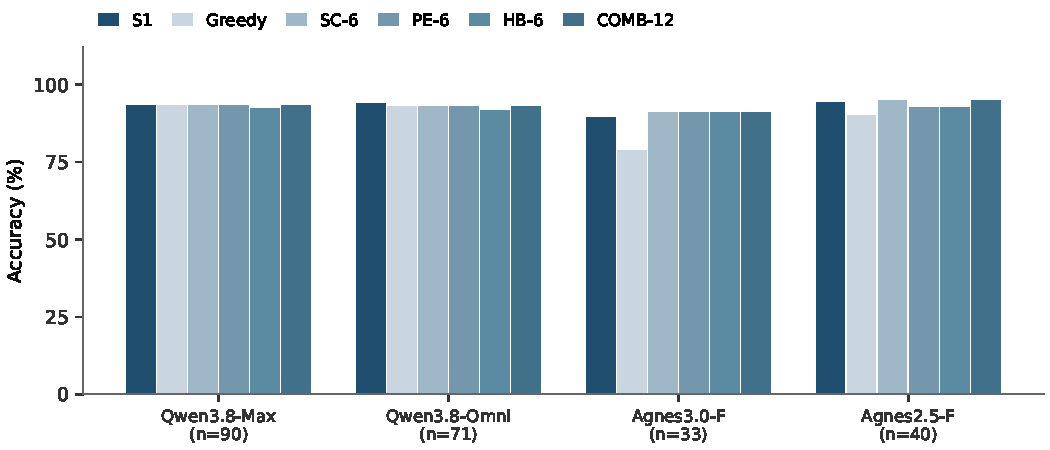
\includegraphics[width=\columnwidth]{figures/conditions.pdf}
\caption{Accuracy of the single-sample baseline S1, the greedy reference, and the four aggregation conditions for the four models with at least twenty complete question matrices. The two Qwen flagships show identical accuracy across conditions, which reflects answer degeneracy rather than agreement between strategies; the models where the modal answer is wrong (GPT-6-Luna, Gemini3.8-Flash) show the two diversity sources pulling in opposite directions. Exact values are given in Table~\ref{tab:main}.}
\label{fig:conditions}
\end{figure}

A separate result concerns the greedy reference itself: greedy decoding at $\tau = 0$ is not an unbiased stand-in for a single stochastic draw. Pooled over the same 112 pairs, S1 reaches 96.4\% against 92.0\% for greedy, a $+4.5$ point gap whose question-level cluster-bootstrap interval, $[+0.9, +8.8]$, excludes zero. The gap is model dependent in both direction and mechanism. For the two Agnes models, greedy sits $10.6$ and $4.2$ points below S1; auditing the discordant questions shows one clear truncation artifact (a greedy chain-of-thought that hit the token cap, after which the parser extracted an intermediate number), two cases of mode locking where the greedy answer differed from every one of the six sampled answers, and remaining cases where greedy picks a minority answer. For GPT-6-Luna and Gemini3.8-Flash the sign reverses ($-3.3$ and $-5.6$ points), and for these models the greedy answer always coincided with the modal sampled answer on our data. Neither baseline subsumes the other, which is why Table~\ref{tab:main} reports both; but because the ensembles aggregate stochastic calls, S1 is the fair comparison, and gains measured against greedy conflate the ensembling effect with the greedy-versus-sampled gap. For a practitioner who currently deploys only greedy decoding, the most direct consequence is a decoding recommendation rather than an ensembling one: on the affected Agnes endpoints, replacing the greedy call with a single stochastic draw at the same budget already recovers four to eleven points in our data. The raw outputs of every audited discordant question --- the truncation artifact, the mode-locking cases, and the minority picks --- are included in the released supplementary material (greedy-bias audit) so that each mechanism can be inspected directly. Section~\ref{sec:heldout} adds the decisive qualification: on the held-out suite, the gap reappears on only one of four endpoints, so the divergence documented here is a property of specific model--endpoint configurations, not a general property of greedy decoding.

Two further observations complete the accuracy picture. The hybrid allocation is a hedge rather than a dominant strategy: it matches the better pure strategy when one source fails, as for GPT-6-Luna where HB-6 and PE-6 both reach 86.7\% while SC-6 falls to 73.3\%, but it never exceeds the better pure strategy on any model, and it trails it by exactly one question on Qwen3.8-Max (92.2 versus 93.3), Qwen3.8-Omni (91.5 versus 93.0), and Agnes2.5-Flash (92.5 versus 95.0). The twelve-vote combined ensemble likewise does not dominate the six-vote conditions: pooled it exactly matches S1 at 96.4\% against 97.3\% for SC-6, because for three of the four pooled models the paraphrase votes it adds are individually no better than a single canonical draw and dilute the majority. Doubling the budget therefore buys no guarantee; the quality of the marginal vote, not the count, governs the outcome.

On the central question, whether one diversity source buys more accuracy per call than the other, no difference is detected in this data against either baseline. Against S1, the pooled SC-6 advantage over PE-6 is $1.8$ points --- two (model, question) pairs out of 112, both resolved in favor of SC-6 --- with a question-level cluster-bootstrap 95\% interval of $[0.0, +5.4]$ (the 90\% interval that the TOST procedure operates on is $[0.0, +3.6]$), and the per-model intervals for the gain over S1 all include zero (Table~\ref{tab:tests}); no per-model McNemar test on the SC-6-versus-PE-6 discordances approaches significance (all $p \ge 0.5$), and the smallest McNemar $p$ anywhere in the table is $0.125$ (SC-6 versus greedy on Agnes3.0-Flash), which does not survive any multiple-comparison correction. We emphasize what this does and does not establish. The TOST procedure at equivalence bounds of $\pm 3$ points does not conclude equivalence for the pooled difference, and the bound itself is coarse at these sample sizes: $\pm 3$ points is 2.7 questions at $n = 90$ and fewer than one question on the smallest sets, so a single flipped question can move the verdict. At these sample sizes the study is powered to detect only large differences; a genuine advantage of either source of up to several points could go unnoticed. The two strategies are therefore not interchangeable in principle, and for two reasons the data show they are not interchangeable in practice either: they disagree on individual questions at measurable rates (Section~\ref{app:rq2}), and their agreement signals catch different errors (Section~\ref{app:rq3}).

\begin{table}[htbp]
\centering
\footnotesize
\caption{Paired comparisons between conditions on the development suite: discordant counts ($b$: first condition right, second wrong; $c$: the reverse), exact McNemar $p$, accuracy difference with 95\% question-resampled bootstrap CI, and the TOST verdict at $\pm 3$ point equivalence bounds. ``no'' means equivalence is not established at this sample size, not that a difference was found.}
\label{tab:tests}
\scriptsize
\begin{tabular*}{\columnwidth}{@{\extracolsep{\fill}} l c l c c c c c c}
\toprule
Model & $n$ & Comparison & $b$ & $c$ & McNemar $p$ & Diff. & 95\% CI & TOST $\pm$3 \\
\midrule
Qwen3.8-Max & 90 & SC-6 $-$ S1 & -- & -- & -- & +0.0 & [0.0,0.0] & -- \\
 &  & PE-6 $-$ S1 & -- & -- & -- & +0.0 & [0.0,0.0] & -- \\
 &  & SC-6 $-$ Greedy & 0 & 0 & 1.000 & +0.0 & [0.0,0.0] & -- \\
 &  & SC-6 $-$ PE-6 & 0 & 0 & 1.000 & +0.0 & [0.0,0.0] & yes \\
\addlinespace
Qwen3.8-Omni & 71 & SC-6 $-$ S1 & -- & -- & -- & -0.9 & [-3.3,1.2] & -- \\
 &  & PE-6 $-$ S1 & -- & -- & -- & -0.9 & [-4.0,1.6] & -- \\
 &  & SC-6 $-$ Greedy & 1 & 1 & 1.000 & +0.0 & [-4.2,4.2] & -- \\
 &  & SC-6 $-$ PE-6 & 1 & 1 & 1.000 & +0.0 & [-4.2,4.2] & yes \\
\addlinespace
Agnes3.0-Flash & 33 & SC-6 $-$ S1 & -- & -- & -- & +1.5 & [-2.5,6.1] & -- \\
 &  & PE-6 $-$ S1 & -- & -- & -- & +1.5 & [-2.5,6.1] & -- \\
 &  & SC-6 $-$ Greedy & 4 & 0 & 0.125 & +12.1 & [3.0,24.2] & -- \\
 &  & SC-6 $-$ PE-6 & 0 & 0 & 1.000 & +0.0 & [0.0,0.0] & yes \\
\addlinespace
Agnes2.5-Flash & 40 & SC-6 $-$ S1 & -- & -- & -- & +0.8 & [0.0,2.5] & -- \\
 &  & PE-6 $-$ S1 & -- & -- & -- & -1.7 & [-5.0,0.0] & -- \\
 &  & SC-6 $-$ Greedy & 2 & 0 & 0.500 & +5.0 & [0.0,12.5] & -- \\
 &  & SC-6 $-$ PE-6 & 1 & 0 & 1.000 & +2.5 & [0.0,7.5] & no \\
\addlinespace
GPT-6-Luna & 15 & SC-6 $-$ S1 & -- & -- & -- & -3.3 & [-12.2,4.4] & -- \\
 &  & PE-6 $-$ S1 & -- & -- & -- & +10.0 & [0.0,22.2] & -- \\
 &  & SC-6 $-$ Greedy & 0 & 1 & 1.000 & -6.7 & [-20.0,0.0] & -- \\
 &  & SC-6 $-$ PE-6 & 0 & 2 & 0.500 & -13.3 & [-33.3,0.0] & no \\
\addlinespace
Gemini3.8-Flash & 12 & SC-6 $-$ S1 & -- & -- & -- & -2.8 & [-12.5,4.2] & -- \\
 &  & PE-6 $-$ S1 & -- & -- & -- & +5.6 & [0.0,13.9] & -- \\
 &  & SC-6 $-$ Greedy & 0 & 1 & 1.000 & -8.3 & [-25.0,0.0] & -- \\
 &  & SC-6 $-$ PE-6 & 0 & 1 & 1.000 & -8.3 & [-25.0,0.0] & no \\
\bottomrule
\end{tabular*}
\end{table}

The comparison is also matched in tokens, not only in calls. Averaged per call, canonical-sample and paraphrase calls cost within one to five percent of each other for every model (for example 223 versus 219 tokens for Qwen3.8-Max and 505 versus 528 for GPT-6-Luna), because validated paraphrases change the surface form but not the length of the task: the mean character-length ratio between paraphrase and original stems is 1.06 for the Qwen models and 1.13 to 1.14 for the API-served models. Budgets matched in calls are therefore approximately matched in cost for this suite.

\subsection{RQ2: Paraphrase fragility}
\label{app:rq2}
\label{sec:rq2}

\emph{In one sentence:} fragility is negligible in the degenerate regime and substantial in the high-entropy regime, and on this suite flips were an entirely stem-locus phenomenon --- a locus split the held-out suite later corrected (Section~\ref{sec:heldoutfragility}).

Fragility, the fraction of questions where paraphrasing alone flips the majority answer, is negligible in the degenerate regime and substantial in the high-entropy regime. Qwen3.8-Max shows fragility on 1.1\% of questions and Qwen3.8-Omni on 4.2\%, concentrated almost entirely in LogiQA, where the respective per-dataset fragility rates are 6.7\% and 21.4\%. The models with high answer entropy on logical reasoning show more: GPT-6-Luna flips on 13.3\% of its questions overall and on 40\% of its LogiQA questions, and Gemini3.8-Flash on 8.3\% overall and 33.3\% of LogiQA. Agnes3.0-Flash, whose gains come with fully consistent votes across both sources, shows zero fragility.

Stratifying by paraphrase locus, which the design fixes in advance, showed flips on this suite to be an entirely stem-locus phenomenon: across all six models, no question flipped under instruction paraphrasing (zero of 52 pooled instruction-locus pairs), while 3.3\% of pooled stem-locus pairs flipped, rising to 28.6\% and 20\% for GPT-6-Luna and Gemini3.8-Flash respectively. The two loci differ by construction in how much of the prompt they vary, so the asymmetry should be read as a property of the perturbation family rather than of the models: instruction rewordings touch only the answer-format scaffolding, while stem rewordings touch the problem content itself. For evaluation practice, the practical consequence is that a single-prompt score on a hard benchmark understates the instability of the measured system by an amount that stem fragility makes visible. The held-out suite, however, shows that the sharper half of this reading was a property of the question draw rather than a structural law: on the fresh questions, instruction-locus flips do occur (9.6\% pooled against 17.4\% for stem-locus), concentrated exactly where the handcrafted instruction variants differ in elicitation quality, on SAT-Math (Section~\ref{sec:heldoutfragility}). Instruction-level paraphrase ensembling therefore probes a weaker axis of variation than stem-level paraphrasing on average, but not a structurally safe one.

Fragility is not random noise; it tracks the same model-task cells that carry answer entropy and ensembling gains, which supports reading it as an observable symptom of unstable knowledge rather than as a formatting artifact. It is also not an artifact of loose paraphrases: recomputing the statistic with only the paraphrases whose fresh embedding similarity exceeds the stricter 0.80 threshold, requiring at least four such paraphrases per question, leaves the rates essentially unchanged or higher for every model (GPT-6-Luna 33.3\% on six qualifying questions versus 13.3\% overall; Gemini3.8-Flash 25.0\% versus 8.3\%; Qwen3.8-Omni 4.8\% versus 4.2\%), so if anything the tighter paraphrases flip more. \ref{app:greedypara} returns to fragility with a decoding-noise-free variant computed from greedy paraphrase decodes, and Section~\ref{sec:heldoutfragility} recomputes the fragility statistics on the held-out suite, where they carry larger denominators and a corrected locus split.

\subsection{RQ3: Consistency as an error signal}
\label{app:rq3}
\label{sec:rq3}

\emph{In one sentence:} on the development suite, models with genuine entropy show informative agreement scores and the stronger source differs across models --- readings that rest on one to three errors and are reported as descriptive only; the held-out recomputation at adequate error counts overturned the sharpest of them (Section~\ref{sec:heldouterror}).

Table~\ref{tab:uncert} evaluates agreement scores as unsupervised detectors of ensemble errors, and Figure~\ref{fig:auroc} visualizes AUROC. Models with fewer than five ensemble errors are marked with a dagger and reported descriptively only; at one to three errors, AUROC values are dominated by individual questions and their confidence intervals would span most of the unit interval. The held-out suite supplies the error counts this analysis needs --- twelve to twenty-one ensemble errors per fully covered model --- and Section~\ref{sec:heldouterror} reports the recomputation; the readings below are the development suite's, and two of them did not survive the recomputation. The pattern follows the regime structure. For the Qwen flagships, where almost every question is degenerate, sample agreement carries almost no signal (AUROC 0.58 for Qwen3.8-Max, 95\% CI $[0.50, 0.78]$) because the score is constant at one for nearly all questions, right or wrong; the degenerate stratum contributes errors that are invisible to any agreement-based detector by construction, and five of Qwen3.8-Max's six errors are missed by both signals. Qwen3.8-Omni retains moderate signal (0.79). In the models with genuine entropy the scores become informative and the stronger source differs across models: for Agnes3.0-Flash, sample agreement reads as highly discriminative (0.96, CI $[0.89, 1.00]$) while paraphrase agreement reads as weak (0.60); for GPT-6-Luna paraphrase agreement is the stronger signal (0.92 against 0.58) and for Gemini3.8-Flash both signals separate its single error perfectly. Agnes2.5-Flash, whose answers are mostly degenerate, shows a reversed sample-agreement ranking that we read as noise at its two-error rate. The Agnes3.0-Flash reading is the one the held-out suite overturned: at eighteen errors the two signals are comparable there (0.80 against 0.81), so the development-suite contrast should be read as an artifact of the three-error denominator, exactly what the five-error rule of Section~\ref{sec:method} was designed to flag.

\begin{table}[htbp]
\centering
\footnotesize
\caption{Uncertainty estimation on the development suite. Error rate of the COMB-12 reference; AUROC of reversed agreement scores for predicting ensemble errors (95\% bootstrap CI where the model has at least five errors); and the area under the risk-coverage curve (AURC; lower is better), computed by accepting questions in decreasing order of confidence with ties broken uniformly at random and averaged over 1{,}000 permutations, so a random ranking yields AURC equal to the error-rate column. Both is the sum of the two disagreement scores (AUROC only). $^\dagger$Fewer than five errors: descriptive only. Dashes indicate constant scores or zero errors.}
\label{tab:uncert}
\footnotesize
\begin{tabular*}{\columnwidth}{@{\extracolsep{\fill}} l c c c c c c}
\toprule
 & & \multicolumn{3}{c}{AUROC} & \multicolumn{2}{c}{AURC$^{\ddagger}$} \\
\cmidrule(lr){3-5}\cmidrule(lr){6-7}
Model & Err. & $c_S$ & $c_P$ & Both & $c_S$ & $c_P$ \\
\midrule
Qwen3.8-Max & 6.7 & 0.583 & 0.576 & 0.578 & 0.057 & 0.058 \\
Qwen3.8-Omni & 7.0 & 0.788 & 0.779 & 0.780 & 0.031 & 0.032 \\
Agnes3.0-Flash$^\dagger$ & 9.1 & 0.961 & 0.600 & 0.922 & 0.009 & 0.073 \\
Agnes2.5-Flash$^\dagger$ & 5.0 & 0.487 & 0.704 & 0.704 & 0.051 & 0.029 \\
GPT-6-Luna$^\dagger$ & 13.3 & 0.577 & 0.923 & 0.769 & 0.105 & 0.024 \\
Gemini3.8-Flash$^\dagger$ & 8.3 & 0.955 & 0.955 & 1.000 & 0.011 & 0.011 \\
\bottomrule
\end{tabular*}
\end{table}

\begin{figure}[htbp]
\centering
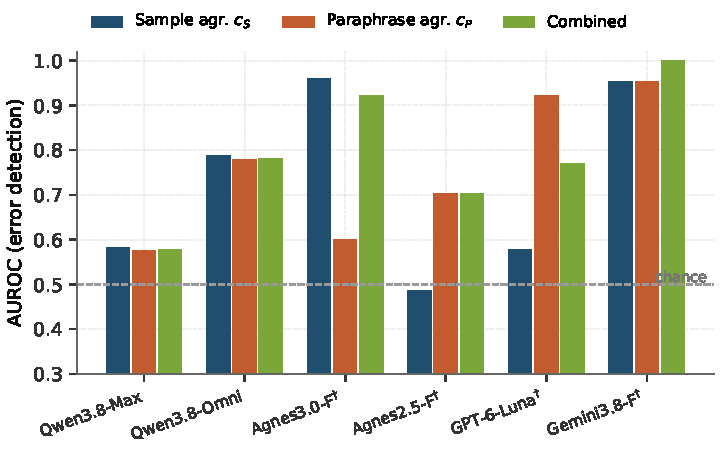
\includegraphics[width=0.8\columnwidth]{figures/auroc.pdf}
\caption{AUROC of reversed agreement scores for detecting ensemble errors. The dashed line marks chance. Signal strength follows the entropy regime, and the stronger source differs across models. $^\dagger$Models with fewer than five errors, reported descriptively.}
\label{fig:auroc}
\end{figure}

The risk-coverage analysis in Table~\ref{tab:uncert} quantifies the selective-prediction value of each signal, with ties in the confidence score resolved by uniformly random tie-breaking (Section~\ref{sec:method}), so each AURC is directly comparable with the model's overall error rate, which is the AURC of a random ranking. Sample agreement attains an AURC of 0.031 for Qwen3.8-Omni against an error rate of 7.0\%, and 0.009 for Agnes3.0-Flash against 9.1\%; paraphrase agreement attains 0.032 and 0.073 on the same models, so the AURC ordering tracks the AUROC ordering, and each value sits below its model's error rate as expected when the ranking carries signal. For Qwen3.8-Max, whose signals are uninformative, AURC stays at 0.057 against a 6.7\% error rate, close to the random baseline as expected. Pooled over the four well-covered models, sample agreement reaches an AUROC of 0.74 (cluster-bootstrap 95\% CI $[0.71, 0.75]$) against 0.60 $[0.46, 0.73]$ for paraphrase agreement, an interval that overlaps chance: pooled across models with opposite signal strengths, the paraphrase signal averages out.

The two agreement scores therefore measure different failure modes, but the evidence for complementarity is about coverage, not about a superior combined detector. Among the ensemble errors of the models with informative signals, the flagged sets overlap only partially: for Agnes3.0-Flash, sample agreement flags all three errors while paraphrase agreement flags one, two of them only through sample agreement; for GPT-6-Luna, paraphrase agreement flags both errors and sample agreement only one; for Qwen3.8-Omni the two signals flag the same three of five errors. Accordingly, the combined Both score exceeds the best single signal only for Gemini3.8-Flash, ties it for Agnes3.0-Flash (0.92 against 0.96 for sample agreement alone, i.e., slightly below), and falls between the two singles elsewhere; pooled it reaches 0.73 against 0.74 for sample agreement alone. A deployment that can afford both probes obtains partially disjoint evidence, and neither signal subsumes the other. On this suite the simple sum of the two disagreement scores does not dominate the best single signal; the held-out suite, at adequate error counts, reversed that reading (Section~\ref{sec:heldouterror}), so we treat the combination question as open rather than settled against the sum, with a learned or calibrated combination remaining the natural next step. We also note the structural caveat of Section~\ref{sec:method}: on questions where all twelve votes coincide, the reference answer equals that unanimous vote by construction, so detectors that read unanimity are correct by definition on the degenerate stratum; the informative content of Table~\ref{tab:uncert} lies in the non-degenerate stratum, which the flagged-error analysis above reflects.

\subsection{RQ4: The regime structure}
\label{app:rq4}
\label{sec:rq4}

\emph{In one sentence:} disagreement predicts the fragility of the greedy reference rather than the value of ensembling; the sign of the ensemble gain is set by whether the modal answer is correct, and high-dissent cells are small and descriptive.

Table~\ref{tab:regime} reports per model and dataset the greedy accuracy, the single-sample expectation, the combined-ensemble accuracy, the gain of the latter over the former, the mean modal vote share, and the mean dissent share (one minus the modal share), and Figure~\ref{fig:regime} plots the ensemble gain over S1 against the dissent share for every model-dataset cell. The scatter shows the dependency that anchors the whole study. Disagreement predicts the fragility of the greedy reference rather than the value of ensembling: across the pooled (model, question) pairs of the four well-covered models, the Spearman rank correlation between the dissent share and the gap $\mathrm{S1} - \mathrm{greedy}$ is $+0.80$, meaning that greedy decoding departs furthest from the sampled consensus exactly where the votes disagree, while the correlation between dissent and the COMB-12 gain over S1 is only $+0.17$: relative to a single stochastic draw, ensembling neither gains nor loses much on average, it only converts an uncertain single draw into the modal answer. Both correlations must be read with their tie structure in mind: 104 of the 112 pooled pairs are unanimous, on them the gap is nonzero exactly once and the COMB-12 answer never differs from S1, so the rank ordering is determined by the eight non-unanimous pairs, within which the gap correlation is $+0.57$; using the absolute gap instead of the signed gap leaves the pooled value unchanged at $+0.80$. Because the combined share and the combined ensemble draw on the same twelve votes, we also recompute the ensemble-gain correlations with strictly disjoint votes: the sample-side dissent share against the PE-6 gain over S1 gives $-0.20$, and the paraphrase-side dissent share against the SC-6 gain over S1 gives $+0.54$, both resting on the same eight informative pairs and read as descriptive. The stratified view makes the structure explicit: the pooled pairs split 104 unanimous, five with a strong majority (share at least two thirds), and three with a weak or no majority. In the unanimous stratum the sampled conditions all sit at 98.1\% (greedy at 97.1\%), and the combined ensemble returns exactly the S1 answer on every one of the 104 unanimous pairs. In the five strong-majority pairs, S1 is 76.7\% and the six-vote ensembles 80.0\%. In the three weak-majority pairs, S1 is 72.2\%, SC-6 reaches 100\%, PE-6 falls to 33.3\%, and the combined ensemble 66.7\%; with three pairs these numbers are descriptive, but they display the full plurality-vote signature of Section~\ref{sec:condorcet}: aggregation pays where the mode is right and is destructive where it is wrong.

\begin{table}[htbp]
\centering
\footnotesize
\caption{Regime map by model and dataset: greedy accuracy, single-sample expectation S1, COMB-12 accuracy, the COMB-12 gain over S1 ($\Delta_C$), the mean modal vote share over the twelve stochastic votes, and the mean dissent share (one minus the modal share, in percent).}
\label{tab:regime}
\scriptsize
\begin{tabular*}{\columnwidth}{@{\extracolsep{\fill}} l l c c c c c c c}
\toprule
Model & Dataset & $n$ & Greedy & S1 & COMB & $\Delta_C$ & Share & Diss.\% \\
\midrule
Qwen3.8-Max & GSM8K & 15 & 100.0 & 100.0 & 100.0 & +0.0 & 100.0 & 0.0 \\
Qwen3.8-Max & SAT-Math & 15 & 100.0 & 100.0 & 100.0 & +0.0 & 100.0 & 0.0 \\
Qwen3.8-Max & PIQA & 15 & 100.0 & 100.0 & 100.0 & +0.0 & 98.9 & 1.1 \\
Qwen3.8-Max & TruthfulQA & 15 & 100.0 & 100.0 & 100.0 & +0.0 & 100.0 & 0.0 \\
Qwen3.8-Max & LSAT-LR & 15 & 100.0 & 100.0 & 100.0 & +0.0 & 100.0 & 0.0 \\
Qwen3.8-Max & LogiQA & 15 & 60.0 & 60.0 & 60.0 & +0.0 & 97.2 & 2.8 \\
\midrule
Qwen3.8-Omni & GSM8K & 15 & 100.0 & 100.0 & 100.0 & +0.0 & 100.0 & 0.0 \\
Qwen3.8-Omni & SAT-Math & 1 & 100.0 & 100.0 & 100.0 & +0.0 & 91.7 & 8.3 \\
Qwen3.8-Omni & PIQA & 11 & 100.0 & 100.0 & 100.0 & +0.0 & 100.0 & 0.0 \\
Qwen3.8-Omni & TruthfulQA & 15 & 93.3 & 96.7 & 93.3 & -3.3 & 96.1 & 3.9 \\
Qwen3.8-Omni & LSAT-LR & 15 & 100.0 & 98.9 & 100.0 & +1.1 & 99.4 & 0.6 \\
Qwen3.8-Omni & LogiQA & 14 & 71.4 & 73.8 & 71.4 & -2.4 & 89.3 & 10.7 \\
\midrule
Agnes3.0-Flash & GSM8K & 7 & 85.7 & 97.6 & 100.0 & +2.4 & 94.0 & 6.0 \\
Agnes3.0-Flash & SAT-Math & 2 & 100.0 & 100.0 & 100.0 & +0.0 & 95.8 & 4.2 \\
Agnes3.0-Flash & PIQA & 5 & 100.0 & 100.0 & 100.0 & +0.0 & 100.0 & 0.0 \\
Agnes3.0-Flash & TruthfulQA & 5 & 100.0 & 100.0 & 100.0 & +0.0 & 100.0 & 0.0 \\
Agnes3.0-Flash & LSAT-LR & 6 & 83.3 & 88.9 & 83.3 & -5.6 & 95.8 & 4.2 \\
Agnes3.0-Flash & LogiQA & 8 & 37.5 & 66.7 & 75.0 & +8.3 & 84.4 & 15.6 \\
\midrule
Agnes2.5-Flash & GSM8K & 7 & 85.7 & 100.0 & 100.0 & +0.0 & 98.8 & 1.2 \\
Agnes2.5-Flash & SAT-Math & 11 & 100.0 & 100.0 & 100.0 & +0.0 & 99.2 & 0.8 \\
Agnes2.5-Flash & PIQA & 7 & 85.7 & 85.7 & 85.7 & +0.0 & 98.8 & 1.2 \\
Agnes2.5-Flash & TruthfulQA & 4 & 100.0 & 100.0 & 100.0 & +0.0 & 100.0 & 0.0 \\
Agnes2.5-Flash & LSAT-LR & 6 & 83.3 & 83.3 & 83.3 & +0.0 & 100.0 & 0.0 \\
Agnes2.5-Flash & LogiQA & 5 & 80.0 & 93.3 & 100.0 & +6.7 & 90.0 & 10.0 \\
\midrule
GPT-6-Luna & GSM8K & 1 & 100.0 & 100.0 & 100.0 & +0.0 & 100.0 & 0.0 \\
GPT-6-Luna & SAT-Math & 5 & 80.0 & 80.0 & 80.0 & +0.0 & 96.7 & 3.3 \\
GPT-6-Luna & PIQA & 2 & 100.0 & 100.0 & 100.0 & +0.0 & 100.0 & 0.0 \\
GPT-6-Luna & TruthfulQA & 2 & 100.0 & 100.0 & 100.0 & +0.0 & 100.0 & 0.0 \\
GPT-6-Luna & LogiQA & 5 & 60.0 & 50.0 & 80.0 & +30.0 & 73.3 & 26.7 \\
\midrule
Gemini3.8-Flash & GSM8K & 1 & 100.0 & 100.0 & 100.0 & +0.0 & 100.0 & 0.0 \\
Gemini3.8-Flash & SAT-Math & 4 & 100.0 & 100.0 & 100.0 & +0.0 & 93.8 & 6.2 \\
Gemini3.8-Flash & PIQA & 2 & 100.0 & 100.0 & 100.0 & +0.0 & 100.0 & 0.0 \\
Gemini3.8-Flash & TruthfulQA & 2 & 100.0 & 100.0 & 100.0 & +0.0 & 100.0 & 0.0 \\
Gemini3.8-Flash & LogiQA & 3 & 66.7 & 44.4 & 66.7 & +22.2 & 66.7 & 33.3 \\
\bottomrule
\end{tabular*}
\end{table}

\begin{figure}[htbp]
\centering
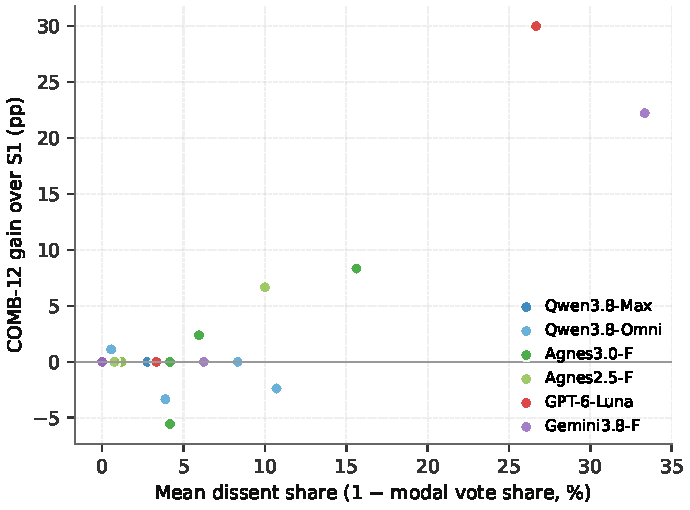
\includegraphics[width=0.75\columnwidth]{figures/regime.pdf}
\caption{Combined-ensemble gain over the single-sample baseline S1 against the mean dissent share (one minus the modal vote share) for every model-dataset cell. Every zero-dissent cell sits exactly at S1. The largest gains sit at the highest dissent: LogiQA under GPT-6-Luna ($+30.0$ points, $n=5$) and LogiQA under Gemini3.8-Flash ($+22.2$, $n=3$), where the sample-side modal answer is wrong while the paraphrase side carries the correct majority into the combined vote. Losses appear at moderate dissent (up to $-5.6$ for LSAT-LR under Agnes3.0-Flash), so the sign of the gain depends on whether the modal answer is correct, not on the amount of disagreement; high-dissent cells contain five questions or fewer, and the pattern is descriptive.}
\label{fig:regime}
\end{figure}

Within the high-dissent region, the two largest gains of the study sit on the two cells with the most dissent, and both are carried by the paraphrase side. Under GPT-6-Luna on LogiQA ($n=5$), the single-sample expectation is 50\%, the six-sample majority drops to 40\% because the modal sampled answer is wrong, while the paraphrase majority rises to 80\% and takes the combined ensemble with it, a $+30.0$ point gain over S1. The LogiQA cell of Gemini3.8-Flash ($n=3$) shows the same signature at smaller scale: S1 is 44.4\%, the sample majority 33.3\%, the paraphrase majority 66.7\%, and the combined ensemble follows it for a $+22.2$ point gain. The plurality-vote model of Section~\ref{sec:condorcet} summarizes the pattern: disagreement is a necessary condition for aggregation to matter at all, but the sign of the gain is determined by which side holds the correct majority, which the dissent share alone does not measure. Both cells are small --- five and three questions --- so we read them as the clearest descriptive illustrations of the mechanism rather than as precise estimates of its size.

The budget curves in Figure~\ref{fig:budget} complete the picture, with the single-sample baseline S1 at $k=1$ and the greedy level marked as a dotted line; panel headers state how many percentage points one question contributes, since a single flipped question moves accuracy by 1.1 to 3.0 points at these sample sizes. For the flagships the curves are flat at the greedy level within one question at every budget, with the one-question deviations reflecting individual tie-breaks rather than trends: Qwen3.8-Max dips one question under PE at $k \in \{2,4\}$, and Qwen3.8-Omni wiggles one question above greedy under SC-4. For Agnes3.0-Flash, the paraphrase ensemble reaches its full 90.9\% already at $k=2$ while the sample majority needs $k=4$ to catch up, the two curves crossing rather than one leading throughout. For Agnes2.5-Flash the ordering is the reverse and persists: sample voting climbs to 95.0\% by $k=6$ while paraphrase voting plateaus at 92.5\%. The practical reading is that the choice between the two sources matters less than the choice of whether to aggregate at all, which the disagreement regime determines, and that neither source dominates the other in budget profile across models.

\begin{figure}[htbp]
\centering
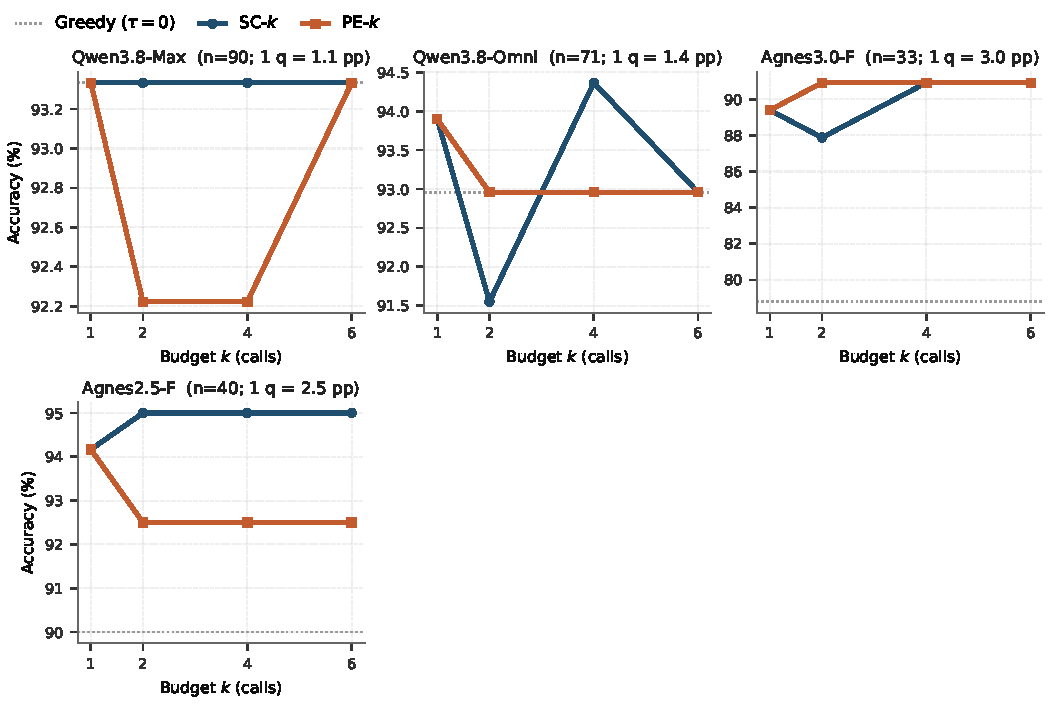
\includegraphics[width=\columnwidth]{figures/budget.pdf}
\caption{Accuracy against call budget $k$ for self-consistency (SC-$k$) and paraphrase ensembling (PE-$k$), with the single-sample baseline S1 at $k=1$ and the greedy accuracy as a dotted line. Panel headers give each model's question count and the accuracy value of one question. Flat curves indicate the degenerate regime; rising or crossing curves indicate cells where aggregation changes answers.}
\label{fig:budget}
\end{figure}

\subsection{Budget efficiency: early stopping and adaptive allocation}
\label{app:efficiency}
\label{sec:efficiency}

\emph{In one sentence:} on the development suite the unanimity rule preserves SC-6 accuracy at two to three calls, and the adaptive rule matches the best fixed strategy on four of six models at 68--78 percent of the budget --- a consistency check, not a validation; the fresh-question transfer test is Section~\ref{sec:heldoutrule}.

The regime structure implies that most of a fixed budget is spent confirming answers that additional calls cannot change. Two simulated policies quantify the waste; both are replays of our own data rather than new methods, and both descend from existing work on sample-adaptive stopping: the sequential unanimity rule is a special case of the early-stopping self-consistency line \citep{aggarwal2023lets,li2024escape}, and we read our simulation as a reproduction of that line's finding in the direct-answering, near-degenerate regime rather than as a novel contribution. The unanimity rule draws canonical samples until the first $k$ at which all drawn samples agree, answers with that unanimous vote, and otherwise falls back to the six-sample majority. The adaptive allocation rule of Section~\ref{sec:discussion} probes each question with two canonical samples and two paraphrases, then routes the remaining budget to paraphrases, resampling, or a split according to which side shows diversity. Table~\ref{tab:efficiency} reports both policies against the fixed conditions, with the probe's calls charged to the adaptive rule; its mean budget runs 4.1 to 4.7 calls, 68 to 78 percent of the six-call budget.

\begin{table}[htbp]
\centering
\footnotesize
\caption{Budget efficiency on the development suite. Accuracy (\%) of the fixed conditions against the sequential unanimity rule (ES, with mean budget $\bar{k}$) and the adaptive allocation rule (Ada, with mean budget and its share of the six-call budget), both simulated on the collected call matrices.}
\label{tab:efficiency}
\scriptsize
\begin{tabular*}{\columnwidth}{@{\extracolsep{\fill}} l c c c c c c c c c}
\toprule
Model & S1 & SC-6 & PE-6 & ES acc & ES $\bar{k}$ & Ada acc & Ada $\bar{k}$ & Budget & COMB-12 \\
\midrule
Qwen3.8-Max & 93.3 & 93.3 & 93.3 & 93.3 & 2.0 & 93.3 & 4.1 & 68\% & 93.3 \\
Qwen3.8-Omni & 93.9 & 93.0 & 93.0 & 93.0 & 2.2 & 91.5 & 4.3 & 71\% & 93.0 \\
Agnes3.0-Flash & 89.4 & 90.9 & 90.9 & 90.9 & 2.5 & 90.9 & 4.6 & 77\% & 90.9 \\
Agnes2.5-Flash & 94.2 & 95.0 & 92.5 & 95.0 & 2.1 & 92.5 & 4.2 & 70\% & 95.0 \\
GPT-6-Luna & 76.7 & 73.3 & 86.7 & 80.0 & 2.0 & 86.7 & 4.5 & 76\% & 86.7 \\
Gemini3.8-Flash & 86.1 & 83.3 & 91.7 & 83.3 & 2.7 & 91.7 & 4.7 & 78\% & 91.7 \\
\bottomrule
\end{tabular*}
\end{table}

The unanimity rule preserves SC-6 accuracy within one question for every model at a mean budget of 2.0 to 2.7 calls, because degenerate questions announce themselves after two or three unanimous draws. The adaptive rule matches the best fixed six-call strategy on four of the six models and trails it by exactly one question on the remaining two, Qwen3.8-Omni (91.5 against 93.0) and Agnes2.5-Flash (92.5 against 95.0), while spending a mean of 4.1 to 4.7 calls, 68 to 78 percent of the six-call budget; it never exceeds the best fixed strategy on any model, and the one-question deficits are exactly the questions whose diversity the two-call probe did not reveal. The comparison against the fixed paraphrase ensemble is the sharpest way to state what the rule adds: the adaptive rule's accuracy equals PE-6's on five of the six models and sits one question below it on Qwen3.8-Omni, so on this data its realized allocation reproduces PE-6 at 68 to 78 percent of its calls. Its increment is the call saving, not accuracy --- the accuracy advantage exists only against a misallocated fixed budget such as SC-6 on GPT-6-Luna --- and on Agnes2.5-Flash it forgoes the one-question edge that fixed SC-6 holds over PE-6 there. A rule worth its added complexity over always running PE-6 must therefore be justified on fresh questions and harder distributions, where the probe's routing can matter in both directions. Because the rule was designed and evaluated on the same collected matrices, this simulation is a consistency check on the rule, not a validation of it; Section~\ref{sec:heldoutrule} performs the fresh-question transfer test. The savings are conservative estimates: the simulation commits to a fixed routing rule after the probe rather than continuing to monitor agreement as later calls arrive, and it charges the full probe even on questions where one call would have sufficed. Both simulations are exact replays of the released call matrices, so they can be re-derived from the logs.
   % A: development-suite details
\section{Greedy paraphrases: isolating the prompt-space effect}
\setcounter{table}{0}
\label{app:greedypara}
\label{sec:greedypara}

The standard paraphrase ensemble decodes each paraphrase once at $\tau = 0.7$, so its diversity mixes prompt-space variation with decoding stochasticity. The greedy-paraphrase control removes the second component by decoding each paraphrase at $\tau = 0$, yielding the noise-free ensemble $\mathrm{PE}^{g}\text{-}6$ and a fragility indicator in which neither side involves sampling. Table~\ref{tab:greedypara} reports the control for the five models whose provider quota allowed it. The control is a development-suite condition: it was not re-collected on the held-out suite, so the held-out paraphrase margins of Section~\ref{sec:expand} retain the mixing that this control removes. Where the control exists, the mixing is small for exactly the family that carries the held-out prompt-space margins --- the two Agnes models show $\mathrm{PE}^{g}$-6 versus PE-6 modal-answer agreement on 31 of 32 and 38 of 39 questions --- while the two DeepSeek endpoints, whose held-out significant conditions are the mixed and combined allocations rather than pure PE-6, have no such measurement, and their prompt-space margins are read with that caveat.

\begin{table}[htbp]
\centering
\footnotesize
\caption{Greedy-paraphrase control. Accuracy (\%) of the greedy baseline, SC-6, PE-6, and the greedy-decoded paraphrase ensemble PE$^{g}$-6; Frag.$^{g}$ is the fraction of questions where SC-6 and PE$^{g}$-6 disagree (no decoding noise on the paraphrase side); Degen.$^{g}$ is the fraction of questions where all six greedy paraphrase answers coincide.}
\label{tab:greedypara}
\footnotesize
\begin{tabular*}{\columnwidth}{@{\extracolsep{\fill}} l c c c c c c c c}
\toprule
Model & $n$ & Greedy & SC-6 & PE-6 & PE$^{g}$-6 & Ident. & Frag.$^{g}$ & Degen.$^{g}$ \\
\midrule
Qwen3.8-Max & 88 & 93.2 & 93.2 & 93.2 & 93.2 & 88/88 & 1.1 & 98.9 \\
Qwen3.8-Omni & -- & \multicolumn{7}{c}{quota exhausted before the control could be run} \\
Agnes3.0-Flash & 32 & 81.2 & 93.8 & 93.8 & 93.8 & 31/32 & 3.1 & 71.9 \\
Agnes2.5-Flash & 39 & 89.7 & 94.9 & 92.3 & 92.3 & 38/39 & 2.6 & 89.7 \\
GPT-6-Luna & 15 & 80.0 & 73.3 & 86.7 & 80.0 & 11/15 & 40.0 & 53.3 \\
Gemini3.8-Flash & 12 & 91.7 & 83.3 & 91.7 & 83.3 & 10/12 & 25.0 & 41.7 \\
\bottomrule
\end{tabular*}
\end{table}

The control separates three effects. First, for the flagship, degeneracy is not a temperature artifact: 98.9\% of Qwen3.8-Max's questions return six identical answers even under greedy decoding of six different paraphrases, and the greedy paraphrase ensemble returns the same answer as the sampled paraphrase ensemble on 88 of 88 questions. The collapse is a property of the model-task pair, not of the sampling distribution around it. Second, for the mid-tier models, the prompt-space effect carries the paraphrase ensemble almost entirely: the PE$^{g}$-6 and PE-6 modal answers coincide on 31 of 32 questions for Agnes3.0-Flash and 38 of 39 for Agnes2.5-Flash, so the stochastic component of PE contributes almost nothing beyond the paraphrases themselves in these cells. Third, for the prompt-brittle models, decoding noise and prompt variation interact: GPT-6-Luna's greedy paraphrase ensemble reaches 80.0\% against 86.7\% for the sampled version with modal-answer agreement on only 11 of 15 questions, and Gemini3.8-Flash 83.3\% against 91.7\% with agreement on 10 of 12, so for the most fragile models the sampled paraphrase ensemble retains a two-to-eight point edge over its noise-free counterpart, and the two ensembles disagree on a quarter of the questions. Fragility itself survives the control in strengthened form: GPT-6-Luna flips on 40.0\% of questions and Gemini3.8-Flash on 25.0\% when both sides are decoded greedily, which rules out sampling noise as the cause of paraphrase-induced flips and locates the instability in the model's response to the prompt's surface form.
  % B
\section{Harder tasks: the MMLU-Pro probe}
\setcounter{table}{0}
\label{app:mmlupro}
\label{sec:mmlupro}

The flagship models saturate five of the six main-suite benchmarks, so the degenerate regime dominates their measurements. The MMLU-Pro probe asks whether a harder distribution restores answer entropy under the same direct-answering protocol. Table~\ref{tab:mmlupro} reports the probe; the coverage caveat is stated up front: on hard quantitative items the direct-answering instruction does not always suppress reasoning, and outputs truncated at the token cap lost extraction on a majority of Qwen3.8-Max's probe calls, leaving six complete questions (eight more with at least four parsed votes); the other models parsed cleanly.

\begin{table}[htbp]
\centering
\footnotesize
\caption{MMLU-Pro probe: greedy accuracy, single-sample accuracy S1, and SC-6 accuracy, with mean support-normalized sample entropy, sample degeneracy rate, and the model's main-suite entropy for comparison.}
\label{tab:mmlupro}
\footnotesize
\begin{tabular*}{\columnwidth}{@{\extracolsep{\fill}} l c c c c c c c}
\toprule
Model & $n$ & Greedy & S1 & SC-6 & Entropy & Degen. & Suite entropy \\
\midrule
Qwen3.8-Max & 6 & 50.0 & 50.0 & 50.0 & 0.153 & 83.3 & 0.018 \\
Agnes3.0-Flash & 8 & 12.5 & 6.2 & 0.0 & 0.937 & 0.0 & 0.162 \\
Agnes2.5-Flash & 13 & 84.6 & 76.9 & 84.6 & 0.241 & 69.2 & 0.055 \\
GPT-6-Luna & 15 & 66.7 & 66.7 & 73.3 & 0.261 & 66.7 & 0.267 \\
\bottomrule
\end{tabular*}
\end{table}

The probe shows that difficulty alone does not determine the regime. GPT-6-Luna, the strongest model with full probe coverage, lands in the high-entropy regime: greedy accuracy 66.7\% with mean entropy 0.26 and a 66.7\% degeneracy rate, and self-consistency lifts it to 73.3\%; at $n = 15$ this 6.6 point difference is the movement of a single question and is reported as directional, not as evidence. Qwen3.8-Max remains essentially degenerate on the probe: its six complete questions are unanimous on five, and seven of the eight questions with at least four parsed votes return a single answer, so for this flagship a ten-option hard benchmark under direct answering still collapses to one answer per question. At the other end, Agnes3.0-Flash collapses into near-uniform guessing: entropy 0.94 with zero degeneracy, greedy accuracy 12.5\%, and a self-consistency majority of 0\% on its eight probe questions; at $n = 8$ these values are one to two questions from chance and are likewise directional, but they are consistent with the plurality-vote failure mode of Section~\ref{sec:condorcet} when the modal answer is wrong. Agnes2.5-Flash answers 84.6\% correctly with partial degeneracy and no aggregation change. The probe is small, and we read it as directional evidence: harder tasks shift models along the entropy axis, but into which regime depends on the model, and the flagship's degeneracy is robust to at least this level of difficulty increase under direct answering.
     % C
\section{Answering mode: direct answer versus chain of thought}
\setcounter{table}{0}
\label{app:cot}
\label{sec:cot}

The main suite answers multiple-choice questions directly, while self-consistency was originally motivated for chain-of-thought reasoning. The CoT condition therefore repeats the greedy baseline, the six-sample self-consistency, and, for stem-locus questions, the paraphrase ensemble under an explicit step-by-step instruction. Table~\ref{tab:cot} reports the condition against the direct-answering cells on the same questions.

\begin{table}[htbp]
\centering
\footnotesize
\caption{Chain-of-thought condition on multiple-choice questions: accuracy under greedy, SC-6, and PE-6 with CoT against the same conditions under direct answering on identical questions (Grd$_{dir}$, SC$_{dir}$, PE$_{dir}$), with mean answer entropy under both modes.}
\label{tab:cot}
\scriptsize
\begin{tabular*}{\columnwidth}{@{\extracolsep{\fill}} l c c c c c c c c c}
\toprule
Model & $n$ & Grd & SC-6 & PE-6 & Grd$_{dir}$ & SC$_{dir}$ & PE$_{dir}$ & H & H$_{dir}$ \\
\midrule
Qwen3.8-Max & 9 & 100.0 & 100.0 & 100.0 & 88.9 & 88.9 & 75.0 & 0.000 & 0.000 \\
Agnes3.0-Flash & 12 & 100.0 & 100.0 & 100.0 & 83.3 & 100.0 & 100.0 & 0.077 & 0.066 \\
Agnes2.5-Flash & 33 & 87.9 & 93.9 & 93.3 & 90.9 & 93.9 & 86.7 & 0.095 & 0.028 \\
GPT-6-Luna & 13 & 92.3 & 100.0 & 100.0 & 84.6 & 76.9 & 100.0 & 0.171 & 0.208 \\
\bottomrule
\end{tabular*}
\end{table}

Chain-of-thought answering raises accuracy where it completes, but it does not dissolve the regime structure. For the flagship subset, CoT lifts Qwen3.8-Max from 88.9\% to 100\% on its nine completed questions while leaving the answer distribution fully degenerate: entropy stays at zero and all six samples agree on every question, so self-consistency remains vacuous. For the mid-tier models, CoT preserves or slightly enlarges diversity: Agnes2.5-Flash holds self-consistency at 93.9\% in both modes on its 33 questions while greedy dips from 90.9\% to 87.9\% and entropy rises from 0.03 to 0.10, Agnes3.0-Flash gains from 83.3\% to 100\% under greedy on its 12 completed questions while remaining largely degenerate, and GPT-6-Luna's self-consistency improves from 76.9\% to 100\% on its 13 completed questions with its paraphrase ensemble at 100\% in both modes. The pattern that survives the mode change is the important one: aggregation gains track the entropy regime in both modes, the degenerate stratum stays degenerate under CoT for the flagship, and the paraphrase side continues to carry signal only where entropy exists. Absolute accuracies are not comparable across modes, the CoT subsets are small, and the slow long-form generations bounded coverage for the rate-limited models, so we read this condition as a robustness check on the regime structure rather than as a mode comparison.
         % D
% Appendix E: claim-evidence map for every quantitative or causal claim made
% in the abstract, the introduction, and the conclusion. Downgraded claims are
% marked; the corresponding audit is re-run by the released script.
\section{Claim--Evidence Map}
\setcounter{table}{0}
\label{app:claims}

\emph{In one sentence:} every quantitative or causal claim in the abstract, the introduction, and the conclusion is listed below with its supporting table, figure, or test, together with the confidence interval where one exists; claims whose evidence is descriptive or post hoc are marked as such.

\begin{table}[htbp]
\centering
\footnotesize
\caption{Claim--evidence map. ``Primary'' marks one of the four designated primary contrasts of Section~\ref{sec:stats} (Holm-adjusted within the family); ``expl.'' marks exploratory evidence (no correction claim); ``post hoc'' marks a selection made on the same data it scores; ``by construction'' marks a structural property of the design rather than an empirical finding.}
\label{tab:claims}
\begin{tabularx}{\textwidth}{@{}p{0.44\textwidth}p{0.30\textwidth}X@{}}
\toprule
Claim (as stated) & Evidence & Status / interval \\
\midrule
Held-out pooled: SC-6 gains $+2.4$ over S1 & Table~\ref{tab:expand}; cluster bootstrap & Primary; CI $+1.1$ to $+3.7$; Holm $p=0.0008$ \\
Held-out pooled: PE-6 gains $+4.9$ over S1 & Table~\ref{tab:expand}; cluster bootstrap & Primary; CI $+2.3$ to $+7.6$; Holm $p<0.0001$ \\
Held-out pooled: COMB-12 gains $+4.1$ over S1 & Table~\ref{tab:expand}; cluster bootstrap & Primary; CI $+2.0$ to $+6.3$; Holm $p<0.0001$ \\
SC-6 and PE-6 statistically inseparable & Table~\ref{tab:expand}; PE$-$SC $+2.5$ & Primary; CI $-0.6$ to $+5.7$; Holm $p=0.14$; ``no detectable difference'', not equivalence \\
$+1.9$ of PE headline is a single-call difficulty offset & Table~\ref{tab:expand_ds} (PE-1 $-$ S1 pooled) & Expl.; decomposition of the same votes \\
Like-for-like aggregation: $+3.0$ (paraphrase side) vs $+2.4$ (resampling) & Table~\ref{tab:expand_ds} ($\Delta$PE, $\Delta$SC pooled) & Expl.; intervals overlap between sources \\
Paraphrase margin concentrates on quantitative tasks; coincides with an instruction effect & Table~\ref{tab:expand_ds} by dataset; instruction-variant analysis (Section~\ref{sec:heldoutmech}) & Expl.; post-hoc variant selection (optimistic ceiling) \\
Best single instruction variant reaches 95.0\% on pooled SAT-Math vs 76.2\% canonical and 91.2\% PE-6 & Per-call logs, six handcrafted variants & Post hoc; same data as the selection \\
SC-6 under the best instruction not run & --- & Absent control; flagged in Section~\ref{sec:heldoutmech} and limitations \\
Agnes3.0-Flash held-out: PE-6 $+7.8$ over S1 & Table~\ref{tab:expand} & Expl. per-model; CI $+2.4$ to $+13.7$ \\
Per-model $\Delta$SC between $-3.3$ and $+2.7$ across both suites & Tables~\ref{tab:main}, \ref{tab:expand_ds} & Expl.; descriptive range \\
Greedy divergence from S1 is endpoint-specific (one of four held-out endpoints; four of ten overall) & Greedy-bias audit; Section~\ref{sec:heldoutgreedy} & Expl.; audit of discordant questions \\
Fragility: 17.4\% stem-locus vs 9.6\% instruction-locus pooled flips (held-out) & Held-out call matrices & Expl.; 41/236 vs 23/240 pairs \\
Pooled error-detection AUROC: sample 0.75, paraphrase 0.74, Both 0.81 & Table~\ref{tab:uncertexp} & CI 0.67--0.84, 0.65--0.83, 0.73--0.89; Both ranking is descriptive (overlapping intervals) \\
Union of the two flagged sets is an upper bound by construction; partial disjointness (15 and 12) is the empirical content & Table~\ref{tab:uncertexp} & By construction / expl. \\
Non-degenerate stratum AUROC falls to 0.49--0.86; 35.1\% vs 3.6\% error rates & Table~\ref{tab:uncertexp}; held-out logs & Expl.; regime signal \\
Adaptive rule: 79--87\% of six-call budget on held-out; exceeds fixed frontier on one model by one question & Table~\ref{tab:expand} (rule replay); Section~\ref{sec:heldoutrule} & Expl.; transfer test of a rule designed on development data \\
Sequential unanimity preserves SC-6 within one question at 2--3 calls & Table~\ref{tab:efficiency} & Expl.; simulation (replay of collected matrices) \\
Degenerate regime: ensembles collapse onto single-call baselines; agreement scores uninformative & Table~\ref{tab:regime}; Figure~\ref{fig:budget}; Table~\ref{tab:uncert} & Partly by construction (unanimous votes), prevalence is empirical \\
First budget-matched within-question comparison, to our knowledge & Section~\ref{sec:related} positioning & Literature claim; cannot be verified exhaustively \\
Every paraphrase vote mixes prompt variation with decoding noise; no held-out greedy-paraphrase control & Section~\ref{sec:conditions}; \ref{app:greedypara} & By design \\
\bottomrule
\end{tabularx}
\end{table}

Claims that were downgraded relative to earlier drafts of this work: (i) ``the stronger error signal tracks the model's stronger diversity source'' --- downgraded after the held-out recomputation (Section~\ref{sec:heldouterror}); (ii) ``instruction-locus flips never occur'' --- downgraded to a property of the development-suite draw (Section~\ref{sec:heldoutfragility}); (iii) ``the paraphrase margin concentrates where answer-space diversity is exhausted'' --- downgraded to the instruction-effect reading, because the SAT-Math cell is dominated by the instruction-variant effect and the best-instruction SC-6 control was not run (Section~\ref{sec:heldoutmech}); (iv) ``TruthfulQA is neutral for the paraphrase side'' --- downgraded to ``retains a small within-condition margin ($+3.1$), reported as a residual prompt-side effect'' (Section~\ref{sec:heldoutmech}).
      % E: claim-evidence map, equivalence-check plan

\bibliographystyle{tmlr}
\bibliography{refs}

\end{document}
